\chapter{RGD Family of Models}

\section{RGD Model}

This section briefly summarizes the workflow of RGB model written in MATLAB. More detail description can be seen in \referencename~\cite{ref:zhang2020a}.  This code is for symmetric full blade which is defined as D1 bit in the paper.  The code calculates coupled PDE and ODE by solving the matrix
\begin{equation}\label{matrix}
  \bm{Adx} + \bm{BX} = \bm{Q}
\end{equation}
where $\bm{dx}$ and $\bm{X}$ are defined as follow:
\vspace{\abovedisplayskip}

\noindent\begin{minipage}{.4\linewidth}
\begin{equation}
\bm{x}=
\begin{bmatrix}
\dot{u} \\
u \\
\psi \\
\dot{\psi} \\
a_1\ \\
\vdots \\
a_N \\
\end{bmatrix}
\end{equation}
\end{minipage}%
\hfill
\begin{minipage}{.4\linewidth}
\begin{equation}
\bm{dx}=
\begin{bmatrix}
\ddot{u} \\
\dot{u} \\
\dot{\psi} \\
\ddot{\psi} \\
\dot{a_1}\ \\
\vdots \\
\dot{a_N} \\
\end{bmatrix}
\end{equation}
\end{minipage}
\vspace{\belowdisplayskip}

The bit trajectory function which is $\overline{h}(\tau, \theta$) is introduced and PDE can be derived from equation:
\begin{equation}\label{PDE}
\frac{\partial \overline{h}}{\partial \tau} + (w_0 + \dot{\psi})\frac{\partial \overline{h}}{\partial \theta}-v_0 = 0
\end{equation}

Equation (\ref{PDE}) is solved by Galerkin-method which approximates $\overline{h}(\tau, \theta$) by using base functions $a_1, a_2, ..., a_N$ (N=25 as default), where $\tau$ is scaled time and $\theta$ is rotation angle of the bit blade. The base functions can be obtained by minimizing the residual which are shown below (please note that all the derivations are for D1-bit):

\begin{equation}\label{GM}
\begin{split}
R &= \left(\frac{n \theta}{2 \pi}-1\right)\dot{u}_b + \frac{n \theta}{2 \pi}\dot{a}_1 + \sum_{k=1}^{N-1}\dot{a}_{k+1}sin\left(\frac{nk\theta}{2}\right) \\ + &(w_0 + \dot{\psi}_0)\left[u_b\frac{n}{2\pi}+a_1\frac{n}{2\pi} + \sum_{k=1}^{N-1}\frac{a_{k+1}nk}{2}cos\left(\frac{nk\theta}{2}\right)\right]
\end{split}
\end{equation}

where n is the number of bit blade. In the paper the blade number is divided to $n_i$, and $n_o$ that are number of inner blades and outer blades, respectively. However, the codes runs for D1 bit and it contains n instead of $n_i and n_o$.

Minimizing $R(\theta, \tau)$ can be acheived by making it orthogonal to the base functions over the domain $\theta \in \left[0, \frac{2\pi}{n_i}\right]$, which results in:

\begin{equation}\label{GM1}
 \int_{0}^{\frac{2\pi}{n}}R(\theta,\tau)\frac{n\theta}{2\pi}d\theta = 0
\end{equation}

and

\begin{equation}\label{GM2}
 \int_{0}^{\frac{2\pi}{n}}R(\theta, \tau)sin\left(\frac{n_im\theta}{2}\right)d\theta=0, m= 1,....,N-1
\end{equation}
where N is the number of Galerkin base functions.

Equation (\ref{GM1})-(\ref{GM2}) represent a system of N first order equations for $a_i, i=1,2,...,N$ that is

\begin{equation}\label{Norder}
  \dot{a}_i = \Phi_i(\dot{u}, u, a_1, ..., a_N), i=1,...,N.
\end{equation}

Which is coupled with the equation of motion (governing equation) which are:

\begin{equation}\label{GE1_}
  \ddot{u} = \psi(\varpi_0 - \varpi)
\end{equation}

\begin{equation}\label{GE2_}
  \ddot{\phi} + \phi = \Gamma_0 - \Gamma
\end{equation}

where 
\begin{equation}\label{GE1}
  \varpi-\varpi_0 = n(\delta_n - \lambda(g(\nu)) - \frac{2\pi v}{w_0}
\end{equation}

\begin{equation}\label{GE2}
  \Gamma-\Gamma_0 = n(\delta_n -\beta \lambda(g(\nu)) - \frac{2\pi v}{w_0}
\end{equation}

and $\delta_n$ is given as:

\begin{equation}\label{deltan1}
  \delta_n = \overline{h}\left(\frac{2\pi}{n}, n\right) + u(\tau)
\end{equation}

$\varpi$, $\Gamma$ represent scaled WOB, TOB, respectively,  $\beta$ is number characterizing bit/rock interaction (generally less than 1). v and w are the scaled axial and angular velocity, respectively that are

\begin{equation}\label{scaled_axial_ve}
  v = v_0 + \dot{u}
\end{equation}
\begin{equation}\label{scaled_angular_vel}
  w = w_0 + \dot{\psi}
\end{equation}

So far we have N+2 equations with N+4 unknowns ($u, \dot(u), \psi, \dot(\psi), a_1, ..., a_N$). and two additional equations are obtained from relationship below:

\begin{equation}\label{axial_dis_vel}
  \dot{u} = \frac{\partial u}{\partial \tau}
\end{equation}
\begin{equation}\label{angular_dis_vel}
  \dot{\psi} = \frac{\partial \psi}{\partial \tau}
\end{equation}

Finally we obtained N+4 equations for the same number of unknowns and represent as linear from of $\bm{Adx} + \bm{BX} = Q$. and solve the equation for given time interval. However, the discontinuity should be investigated every time step which affects the boundary condition from rock-bit interaction. The model classifies the discontinuity to three which are 1) normal drilling, 2) axial stick, and 3) bit bonce. Below summarizes the conditions for each mode:

\begin{equation}\label{drillingmodes}
  \begin{cases}
    Normal\,drilling, & \mbox{if $\delta_n > 0, w > 0$, and $v > 0$ }  \\
    Axial\, stick, & \mbox{if $\delta_n >0, w > 0$, and $v = 0$ } \\
    Bit\,bounce, & \mbox{if $\delta_n = 0$, and $w > 0$}
  \end{cases}
\end{equation}

\section{Normal Drilling}
Normal drilling mode simplifies the equations (\ref{GE1}), and (\ref{GE2}) since g($\nu$) = 0 which can be represented as:

\begin{equation}\label{GE1_normaldrilling}
  \varpi-\varpi_0 = n\left(\delta_n - \frac{2\pi v}{w_0}\right)
\end{equation}

\begin{equation}\label{GE2_normaldrilling}
  \Gamma-\Gamma_0 = n\left(\delta_n - \frac{2\pi v}{w_0}\right)
\end{equation}

Also, the depth of cut (\ref{deltan1}) is reduced to:

\begin{equation}\label{deltan_normaldrilling}
  \delta_n = a_1 + u(\tau)
\end{equation}

Afterwards, equation (\ref{matrix}) can be solved with reduced equations from equations (\ref{GE1_normaldrilling}) - (\ref{deltan_normaldrilling})

\newpage
\section{Extended RGD Model (Zhang and Detournay, 2022)}


This section summarizes the paper from Zhang and Detournay 2022, which is an extension of RGD model. The proposed model is a multi-degrees of freedom (MDOF) model of a rotary drilling system simulating axial-torsional self-excited vibrations induced by the bit/rock interactions. \figurename~\ref{model_develop_figure} illustrates the development of the RGD model.

\begin{figure}[ht]
  \centering
  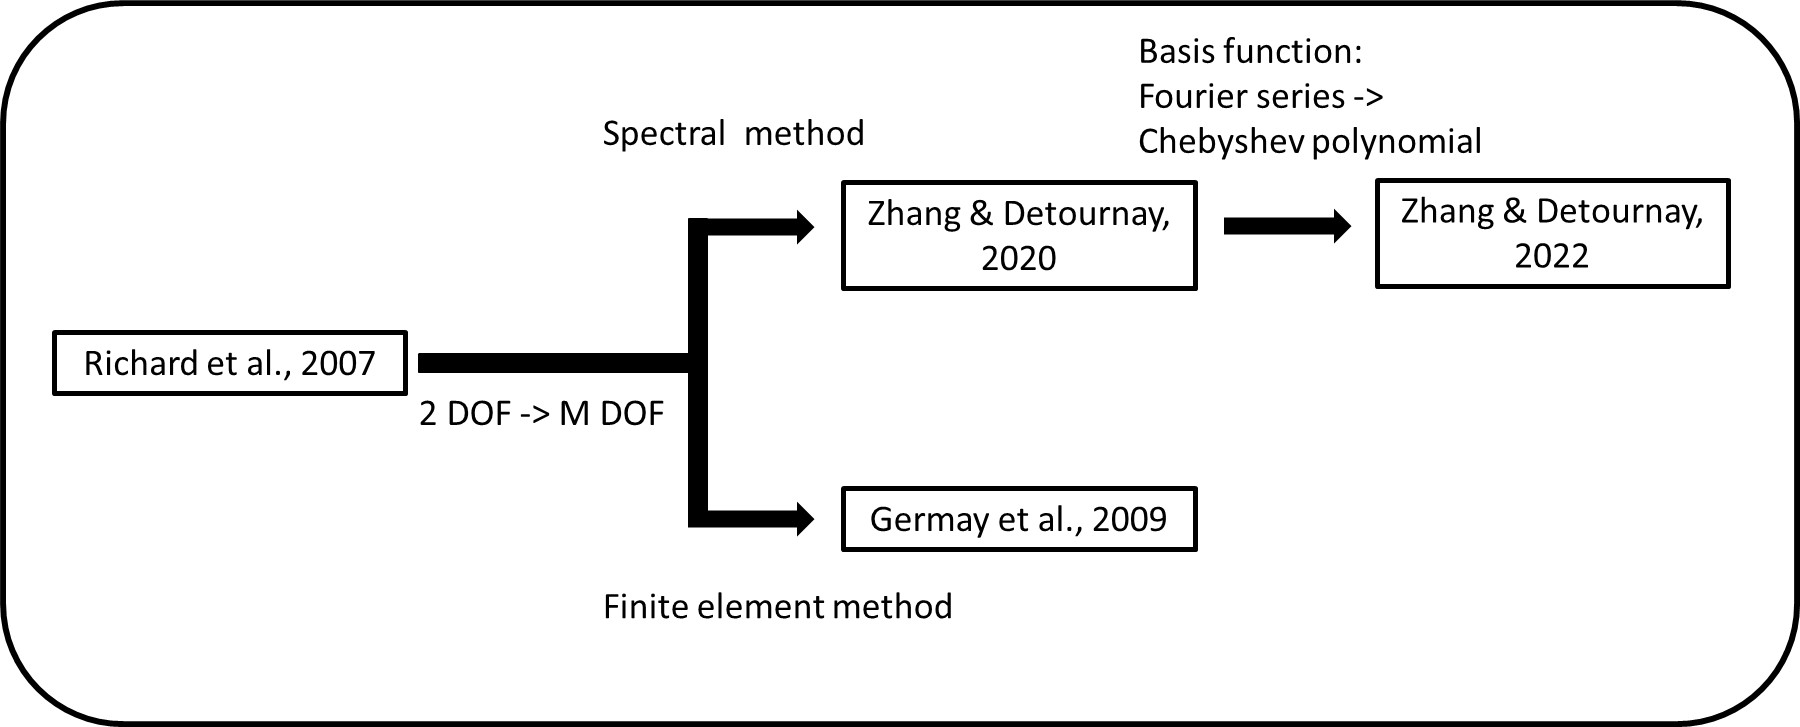
\includegraphics[width=5in]{ModelDevelop}
  \caption[RGD model development]{RGD model development.}\label{model_develop_figure}
\end{figure}

The model represents the drillstring with multiple damped axial and torsional oscillators and the bit with symmetrically arranged blades. The schematic of MDOF model of the drillstring is shown in Figure \ref{MDOF_illustration}. The model takes into account damping and
different properties of drill pipe and BHA

\begin{figure}[ht]
  \centering
  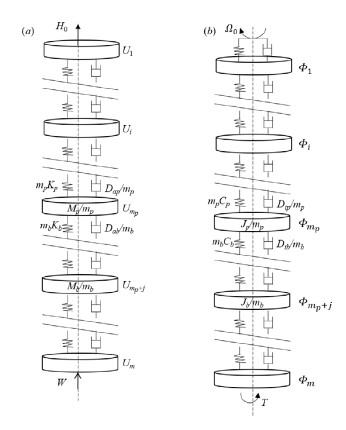
\includegraphics[height=3in]{MDOF_illustration}
  \caption[Schematic of the MDOF model of the drillstring]{Schematic of the MDOF model of the drillstring. a) axial, b) torsional.}\label{MDOF_illustration}
\end{figure}

The following assumptions are made: 1) The borehole is vertical, 2) Lateral vibration of the drillstring are neglected, 3) axial and torsional damping are proportional to the length of drill pipes and BHA, 4) constant hook load and rotary speed from surface (surface boundary conditions). Additionally, the discontinuity of the boundary condition at the bit-rock interface is modeled by
five different regimes classified based on axial, angular velocities, and depth-of-cut, namely, 1) normal drilling, 2) axial stick, 3) loss of contact, 4) torsional stick, 5) backward rotation
The system equations (PDE-ODE coupled) are established from equation of motions (axial and torsional), and bit trajectory function, which is defined to project depth of cut from the angular displacement of the bit. Then,
The PDE-ODE coupled system is numerically solved by discretizing the PDE-ODEs into ODEs. In this study, spectral method with Chebyshev polynomial is applied rather than finite element (FEM) or finite different method (FDM). Spectral method achieved high accuracy for a given number of basis functions and also converged faster compared to other numerical methods. (this is valid with simple geometry). 

Some of the results and potential of the model are summarized below.
\begin{bulletedlist}
  \item Modeling the vibrations of entire drillstring (not only the bit).
  \item Possible to conduct frequency analysis since it is multi-degrees of freedom model (\figurename~\ref{StickslipExample}).
  \item It can simulate axial and torsional vibrations including stick-slip event (\figurename~\ref{Axial_torsional_vibration_example}).
  \item Mode analysis can be done by computing the eigenvalues of the linearized system of equation.
  \item Computationally efficient compared to FEM assuming geometrically simple structure.
\end{bulletedlist}

\begin{figure}[ht]
  \centering
  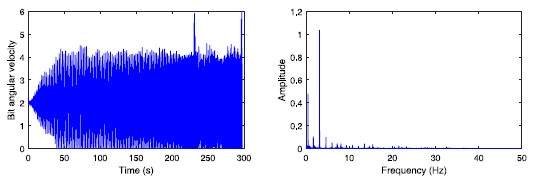
\includegraphics[width=6in]{StickslipExample}
  \caption[Simulation results of bit angular velocity and its frequency spectrum]{Simulation results of bit angular velocity and its frequency spectrum. The result shows the stick-slip occupance due to self-excited torsional vibration}\label{StickslipExample}
\end{figure}


\begin{figure}[ht]
  \centering
  \includegraphics[height=5in]{Axial_torsional_vibration_example}
  \caption[Simulation results showing axial and angular velocity with scaled time]{Simulation results showing axial and angular velocity with scaled time. a) stable regime, b) slow regime of instability, c) fast regime of instability.}\label{Axial_torsional_vibration_example}
\end{figure}

\noindent The following are key questions or points that should be addressed for the model selection.
\begin{bulletedlist}
  \item Can we model deviated or horizontal well?
  \item Geometrical nonlinearity in drillstring (for deviated well).
  \item Can we take int to account the effect of contact point?
  \item No lateral vibration - only modeling axial, torsional motion.
  \item Decoupling of axial and torsional vibration. this can be important when it comes to 3D model (i.e., whirling effect).
  \item Current code provided is 2 DOF model.
\end{bulletedlist} 

\chapter{Aarsnes-Shor Model}

\section{Aarsnes-Shor Model}

The proposed model applies the distributed model of the drillstring with the Coulomb friction given as distributed source term. Most of the previous studies explained the stick-slip behaviour from bit-rock interaction \referencename~\cite{ref:germay2009a, ref:richard2007a, ref:zhang2020a}. Therefore theses models could not validate the stick-slip behavior while off bottom state (i.e., back reaming). The proposed model simulates the torsional stick-slip by take in to account Coulomb-type friction throughout the drillstring. The effect of the distributed, along-string, Coulomb friction becomes prominent of torsional drill string dynamics in wellbores with high-inclination laters. The model was validated with field data from rotational startups, off bottom rotation (without any axial movement), after connection.

Assumptions of the model are listed below:
\begin{bulletedlist}
    \item No bit-rock interaction
    \item No lateral and axial motion
    \item the effects of cuttings distribution on the friction is homogeneous
    \item The transition from static to dynamic coulomb friction is modeled as a jump
\end{bulletedlist}


\noindent Mathematical procedure is summarized below (follows the code flow provided):

The model is based on the equations of angular motion, here named wave equation, which is:
\begin{equation}\label{AS-motion}
  J\rho\frac{\partial w(t,x)}{\partial t} + \frac{\partial \tau (t,x)}{\partial x} = S(w,x) 
\end{equation}

\begin{equation}
 \frac{\partial\tau(t,x)}{\partial t} + JG\frac{\partial w(t,x)}{\partial x} = 0 
\end{equation}

where J is polar moment of inertia and $\rho$ is material density, $w(t,x)$ is angular velocity, $\tau(t,x)$ is torque, and S is the source term which can be represented as:
\begin{equation}\label{AS-sourceterm}
  S(w,x) = -k_t \rho J w(t,x) - \mathcal{F}(w,x)
\end{equation}
where $k_t$ is damping constant which is viscous shear stresses from drilling mud and cuttings bed, and $\mathcal{F}(w,x)$ is Coulomb friction between the drill string and the borehole. 
The 
The partial wave equation is transformed into their Riemann invariants and it is solved by first order upwind scheme. The Riemann invariants are defined as:
\begin{equation}\label{AS-Riemann}
  \alpha = w + \frac{c_t}{JG}\tau, \quad \beta=w-\frac{c_t}{JG}\tau
\end{equation}
where $c_t = \sqrt{\frac{\rho}{J}}$ is the velocity of the torsional wave. and the variable $\alpha, \beta$ satisfies the PDE system below:
\begin{equation}\label{AS-Riemann_alpha}
  \frac{\partial \alpha}{\partial t} + c_t\frac{\partial \alpha}{\partial x} = -\mathcal{S}
\end{equation}
\begin{equation}\label{AS-Riemann_beta}
  \frac{\partial \beta}{\partial t} - c_t\frac{\partial \beta}{\partial x} = -\mathcal{S}
\end{equation}

where the source term $\mathcal{S}$ is
\begin{equation}\label{AS-source}
  \mathcal{S} = \frac{S}{J \rho} j= k_t(\alpha + \beta) + \frac{1}{J \rho} \mathcal{F}
\end{equation}
The boundary conditions are given as:
\begin{equation}\label{AS-BC}
  w_{p,top} = w_{TD} \quad \tau_{c,bottom} = \tau_{bit}
\end{equation}
where subscript p, c represents drill pipe and drill collar.
Additionally, the conditions at the drill pipe - drill collar interface are imposed:
\begin{equation}\label{AS-interface}
  w_{p,interface} = w_{c,interface}, \quad \tau_{p,interface} = \tau_{c,interface}
\end{equation}
\equationname~\ref{AS-BC} and \ref{AS-interface} in Riemann invariants can be written as:
\begin{equation}\label{AS-riemannBC}
  \alpha_{p,top} = -\beta_{p,top} + 2*w_{TD}, \quad \beta_{c,bottom} = \alpha_{c,bottom} - 2\tau_{bit} \frac{c_t}{J_c G_c}
\end{equation}
**Have to check the equation above... This boundary condition seems to take into account the torque from the bit**
\begin{equation}\label{AS-riemanninterface}
\begin{split}
    & \beta_{p,bottom} = \frac{1}{1+\overline{Z}}\left(\alpha_{p,bottom}(1-\overline{Z}) + 2\overline{Z}\beta_{c,top} \right) \\
    & \alpha_{c,top} = \frac{1}{1+\overline{Z}}\left(2*\alpha_{p,bottom} - \beta_{c,top}(1-\overline{Z})\right)
\end{split}
\end{equation}
where $\overline{Z}$is the relative magnitude of the impedance (assuming same $c_t$ for drill pipe and collar - ** need to be checked** ):
\begin{equation}\label{AS_Zbar}
  \overline{Z} = \frac{J_c G_c}{J_p G_p}
\end{equation}

\figurename~\ref{AS_discretizeDS} illustrates the schematic view of the discretized drillstring with boundary conditions, and interface conditions in terms of Riemann invariants. The boundary conditions at the top and bottom of the drillstring are applied to $\alpha$, and $\beta$, respectively. However, since the two variables are coupled by interface conditions, the PDE can be solved. 
The PDE is solved from upwind scheme according to (for sell size $\Delta x$ and time step $\Delta t$, at cell j and time step k):
\begin{equation}\label{AS-upwind}
  \mathcal{F}_{j}^k = \frac{1}{2 \Delta t}\left(a_j^k - c_t \frac{\Delta t}{\Delta x}(a_j^k - a_{j-1}^k) + \beta_j^k + c_t \frac{\Delta t}{\Delta x}(\beta_{j+t}^k-\beta_j^k) + \Delta t k_t (\alpha_j^k + \beta_j^k)\right)
\end{equation}
** There are some difference between code and paper **
\newpage
\begin{figure}[ht]
  \centering
  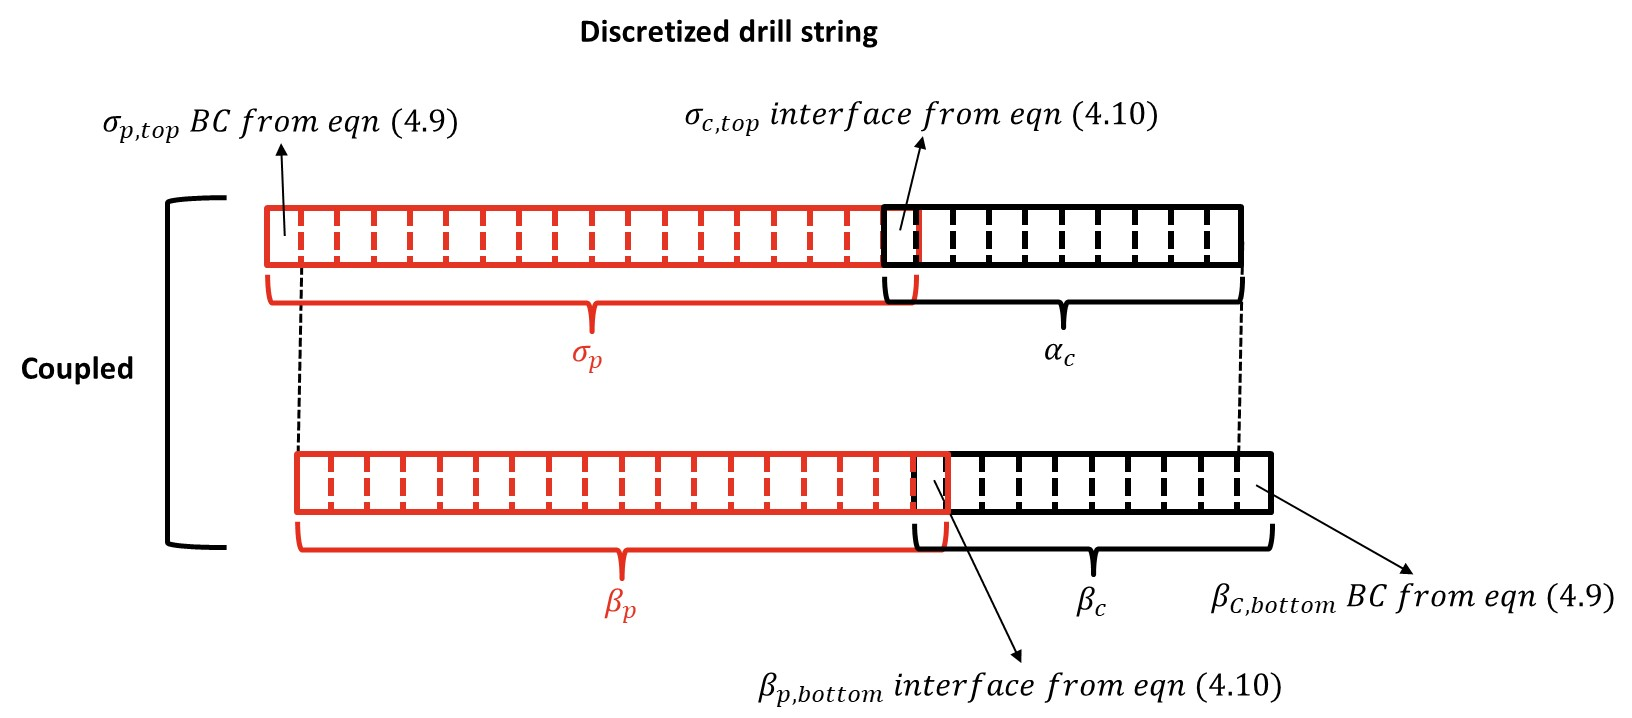
\includegraphics[width=6in]{AS_discretizedDS}
  \caption[Schematic of discretized drillstring and boundary conditions]{Schematic of discretized drillstring, boundary conditions, and interface conditions based on Riemann invariants $\alpha$, and $\beta$.}\label{AS_discretizeDS}
\end{figure}
\section{Aarsnes-Shor Mode - PYTHON}
This section briefly summarizes the code flow (PYTHON version), since it is slightly different in the way they calculated compared to the MATLAB version. The input for torsional modeling is summarized in \tablename~\ref{AS_inptut_params}.

\begin{table}[!hbt]
\centering
\begin{tabular}{|c|c|c|c|c|c|}
\hline
Parameter & Units & Notes\\                                                              
\hline
Simulation length & s & Total simulation time \\                                                  
\hline
Bit depth & ft & MD of the bit \\                                                   
\hline
$w_c$ & rad/s & Cut-off angular velocity (static, dynamic transition)\\                                                              
\hline
$\mu_s$ & -& Static friction factor\\
\hline
$\mu_k$ & - & Kinetic friction factor \\ 
\hline
$K_t$ &- & Inertial torsional damping \\                                                  
\hline
$K_s$ &- & Viscous damping coefficient \\                                                   
\hline
$\rho$ & $lbf/ft_3$ & Drill string density \\                                                       
\hline
G & $lbf/ft^2$ & Shear modulus   \\                                                         
\hline
E & $lbf/ft^2$ & Young's modulus \\                                                              
\hline
$K_p$ & $lb$-$ft$ & P-gain of top drive (PI controller) \\
\hline
$K_i$ & $lb$-$ft/s$ &I-gain of top drive (PI controller)\\ 
\hline
$J_{TD}$ & $lb$-$ft^2$ & Top drive inertia \\
\hline
ramp speed & RPM/s & ramp speed of top drive\\
\hline
\end{tabular}
\caption[Input parameters of Aarsnes-Shor model]{Input parameters of Aarsnes-shor model. well trajectory, top drive set velocity, and bit constant are the additional parameters which are not included in this table.}\label{AS_inptut_params}
\end{table}

First, the static behavior is calculated after descritizing the drillstring. Since the model assumes the off-bottom scenario, WOB and TOB is zero. The normal force, tension, and momentum throughout the drillstring is calculated (Johancsik et al., 1984). Then, the angular velocity, torque is calculated by iterating untill the desired simulation length reaches. The calculation procedure is shown below: 

%\begin{algorithm}
%\caption{Aarsnes-Shor model pseudocode algorithm}\label{AS-pseudocode}
%\begin{algorithmic}
%\For{\texttt{i = 1: simulation length/dt}}
%\State nstep = freq/dt
%\For{\texttt{j=1:nstep}}
%    \State 1. Set the topdrive setpoint torque and angular velocity
%    \State $w_{SP}(t+1)=w_{SP}(t)\pm ramp*dt$
%    \State $e=w_{SP}(t+1)-w_{TD}(t), \quad I=e*dt$
%    \State $\tau_{TD}(t+1) \gets \tau_{TD}(t) + (k_e e + k_i I)*dt$
%    \State $w_{TD}(t+1) \gets w_{TD}(t) + (\tau_{TD}(t+1)-\tau_{top}(t))/J_{TD}*dt$
%    \State 2. Bit rotation
%    \State $\tau_{bit}(t+1) \gets bitconstant * w_{bottom}(t)$
%    \State $w_{bit}(t+1) \gets w_{bottom}(t)$
%    \State 3. Update topdrive torque (?)
%    \State $\tau_{TD}(t+1) \gets \tau_{TD}(t+1)-J_{TD}(w_{TD}(t+1)-w_{TD}(t))/dt$
%    \State 3. Calculate source term
%    \State $fric \gets \mu_k*f_n*r (friction)$
%    \State $Iner \gets k_t*\rho*J*(w(t)-w(t-1)) (intertia\:damping)$
%    \State $vis \gets k_s*w(t) (viscous\:damping)$
%    \State $S \gets (fric+iner+vis)/dx$
%    \State 4. Update the torque and angular velocity \Comment{eqn.\ref{AS-motion}}
%    \State $\tau(t+1) \gets \tau(t) - JG*dl/dt (w_n(t)-w_(n-1)(t))$ \Comment{n is discretized number}
%    \State $w(t+1) \gets w(t) 2*dt/(J*\rho)\left[(\tau_n(t)-\tau_{n-2}(t))/(2*dx)+S\right]$
%    \EndFor
%\State $\overline{w} \gets \overline{w} \cdot Kernel$ \Comment{remove high frequency noise}
%\State $\overline{\tau} \gets \overline{\tau} \cdot Kernel$
%\EndFor
%
%\end{algorithmic}
%\end{algorithm}

\newcommand{\codecomment}[1]{\hfill #1}
\pushinitialcodeindent{0in}

\begin{code}[\codenumbering]{}
\codeitemnonumber \pseudocodefor{} i = 1 simulation length/dt
	\stepcodelevel{}
	\codeitemnonumber nstep = freq/dt
	\codeitemnonumber \pseudocodefor{} {j=1:nstep}
		\stepcodelevel{}
	    \codeitemnonumber 1. Set the topdrive setpoint torque and angular velocity
	    \codeitemnonumber $w_{SP}(t+1)=w_{SP}(t)\pm ramp*dt$
	    \codeitemnonumber $e=w_{SP}(t+1)-w_{TD}(t), \quad I=e*dt$
	    \codeitemnonumber $\tau_{TD}(t+1) \gets \tau_{TD}(t) + (k_e e + k_i I)*dt$
	    \codeitemnonumber $w_{TD}(t+1) \gets w_{TD}(t) + (\tau_{TD}(t+1)-\tau_{top}(t))/J_{TD}*dt$
	    \codeitemnonumber 2. Bit rotation
	    \codeitemnonumber $\tau_{bit}(t+1) \gets bitconstant * w_{bottom}(t)$
	    \codeitemnonumber $w_{bit}(t+1) \gets w_{bottom}(t)$
	    \codeitemnonumber 3. Update topdrive torque (?)
	    \codeitemnonumber $\tau_{TD}(t+1) \gets \tau_{TD}(t+1)-J_{TD}(w_{TD}(t+1)-w_{TD}(t))/dt$
	    \codeitemnonumber 4. Calculate source term
	    \codeitemnonumber $fric \gets \mu_k*f_n*r (friction)$
	    \codeitemnonumber $Iner \gets k_t*\rho*J*(w(t)-w(t-1)) (intertia\:damping)$
	    \codeitemnonumber $vis \gets k_s*w(t) (viscous\:damping)$
	    \codeitemnonumber $S \gets (fric+iner+vis)/dx$
	    \codeitemnonumber 5. Update the torque and angular velocity \codecomment{eqn.\ref{AS-motion}}
	    \codeitemnonumber $\tau(t+1) \gets \tau(t) - JG*dl/dt (w_n(t)-w_(n-1)(t))$ \codecomment{n is discretized number}
	    \codeitemnonumber $w(t+1) \gets w(t) 2*dt/(J*\rho)\left[(\tau_n(t)-\tau_{n-2}(t))/(2*dx)+S\right]$
	    \prevcodelevel{}
	\codeitemnonumber \pseudocodedonefor{}
	\codeitemnonumber $\overline{w} \gets \overline{w} \cdot Kernel$ \codecomment{remove high frequency noise}
	\codeitemnonumber $\overline{\tau} \gets \overline{\tau} \cdot Kernel$
	\prevcodelevel{}
\codeitemnonumber \pseudocodedonefor{}
\end{code}
\popinitialcodeindent{}
\begin{figure}[!hbt]
  \centering
  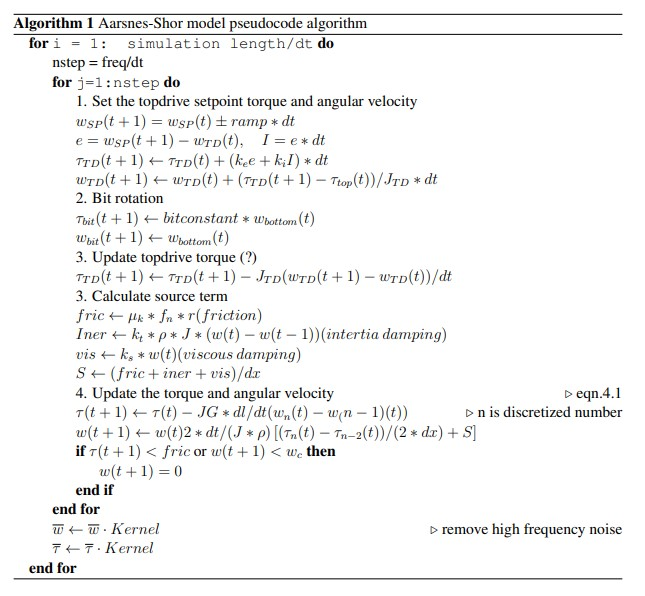
\includegraphics[width=6in]{algorithm_ASmodel}
\end{figure}


%\end{figure}
%\begin{algorithm}
%\caption{Aarsnes-Shor model pseudocode algorithm}\label{AS-pseudocode}
%\begin{algorithmic}
%\For{\texttt{i = 1: simulation length/dt}}
%\State nstep = freq/dt
%\For{\texttt{j=1:nstep}}
%    \State 1. Set the topdrive setpoint torque and angular velocity
%    \State $w_{SP}(t+1)=w_{SP}(t)\pm ramp*dt$
%    \State $e=w_{SP}(t+1)-w_{TD}(t), \quad I=e*dt$
%    \State $\tau_{TD}(t+1) \gets \tau_{TD}(t) + (k_e e + k_i I)*dt$
%    \State $w_{TD}(t+1) \gets w_{TD}(t) + (\tau_{TD}(t+1)-\tau_{top}(t))/J_{TD}*dt$
%    \State 2. Bit rotation
%    \State $\tau_{bit}(t+1) \gets bitconstant * w_{bottom}(t)$
%    \State $w_{bit}(t+1) \gets w_{bottom}(t)$
%    \State 3. Update topdrive torque (?)
%    \State $\tau_{TD}(t+1) \gets \tau_{TD}(t+1)-J_{TD}(w_{TD}(t+1)-w_{TD}(t))/dt$
%    \State 3. Calculate source term
%    \State $fric \gets \mu_k*f_n*r (friction)$
%    \State $Iner \gets k_t*\rho*J*(w(t)-w(t-1)) (intertia\:damping)$
%    \State $vis \gets k_s*w(t) (viscous\:damping)$
%    \State $S \gets (fric+iner+vis)/dx$
%    \State 4. Update the torque and angular velocity \Comment{eqn.\ref{AS-motion}}
%    \State $\tau(t+1) \gets \tau(t) - JG*dl/dt (w_n(t)-w_(n-1)(t))$ \Comment{n is discretized number}
%    \State $w(t+1) \gets w(t) 2*dt/(J*\rho)\left[(\tau_n(t)-\tau_{n-2}(t))/(2*dx)+S\right]$
%    \If{$\tau(t+1)<fric$ or $w(t+1)<w_c$}
%    \State $w(t+1) = 0$
%    \EndIf
%    \EndFor
%\State $\overline{w} \gets \overline{w} \cdot Kernel$ \Comment{remove high frequency noise}
%\State $\overline{\tau} \gets \overline{\tau} \cdot Kernel$
%\EndFor
%\end{algorithmic}
%\end{algorithm}

%\newcommand{\codecomment}[1]{\hfill #1}
%\pushinitialcodeindent{0in}
%
%\begin{code}[\codenumbering]{}
%\codeitemnonumber \pseudocodefor{} {\texttt{i = 1: simulation length/dt}}
%	\stepcodelevel{}
%	\codeitemnonumber nstep = freq/dt
%	\pseudocodefor{} {\texttt{j=1:nstep}}
%		\stepcodelevel{}
%	    \codeitemnonumber 1. Set the topdrive setpoint torque and angular velocity
%	    \codeitemnonumber $w_{SP}(t+1)=w_{SP}(t)\pm ramp*dt$
%	    \codeitemnonumber $e=w_{SP}(t+1)-w_{TD}(t), \quad I=e*dt$
%	    \codeitemnonumber $\tau_{TD}(t+1) \gets \tau_{TD}(t) + (k_e e + k_i I)*dt$
%	    \codeitemnonumber $w_{TD}(t+1) \gets w_{TD}(t) + (\tau_{TD}(t+1)-\tau_{top}(t))/J_{TD}*dt$
%	    \codeitemnonumber 2. Bit rotation
%	    \codeitemnonumber $\tau_{bit}(t+1) \gets bitconstant * w_{bottom}(t)$
%	    \codeitemnonumber $w_{bit}(t+1) \gets w_{bottom}(t)$
%	    \codeitemnonumber 3. Update topdrive torque (?)
%	    \codeitemnonumber $\tau_{TD}(t+1) \gets \tau_{TD}(t+1)-J_{TD}(w_{TD}(t+1)-w_{TD}(t))/dt$
%	    \codeitemnonumber 4. Calculate source term
%	    \codeitemnonumber $fric \gets \mu_k*f_n*r (friction)$
%	    \codeitemnonumber $Iner \gets k_t*\rho*J*(w(t)-w(t-1)) (intertia\:damping)$
%	    \codeitemnonumber $vis \gets k_s*w(t) (viscous\:damping)$
%	    \codeitemnonumber $S \gets (fric+iner+vis)/dx$
%	    \codeitemnonumber 5. Update the torque and angular velocity \codecomment{eqn.\ref{AS-motion}}
%	    \codeitemnonumber $\tau(t+1) \gets \tau(t) - JG*dl/dt (w_n(t)-w_(n-1)(t))$ \codecomment{n is discretized number}
%	    \codeitemnonumber $w(t+1) \gets w(t) 2*dt/(J*\rho)\left[(\tau_n(t)-\tau_{n-2}(t))/(2*dx)+S\right]$
%	    \prevcodelevel{}
%	\codeitemnonumber \pseudocodedonefor{}
%	\codeitemnonumber $\overline{w} \gets \overline{w} \cdot Kernel$ \codecomment{remove high frequency noise}
%	\codeitemnonumber $\overline{\tau} \gets \overline{\tau} \cdot Kernel$
%	\prevcodelevel{}
%\codeitemnonumber \pseudocodedonefor{}
%\end{code}
%\popinitialcodeindent{}

\section{Model Comparison}

\subsection{Case 1 - vertical well}

Exxon mobil model and Aarsnes-shor model (MATLAB ver. and PYTHON ver.) are compared with simple well and drill string configurations. The model parameters and schematic of the wellbore surveys and drill string components are shown in Table \tablename~\ref{table_verticalwell_input}., and Figure \figurename~\ref{figure_verticalwell}. The Exxon mobil model and MATLAB ver. A-S model uses metric units while PYTHON ver. A-S model uses imperial units. For the future convenience, the Table in this chapter contains both imperial and metric units.

\begin{figure}[!hbt]
  \centering
  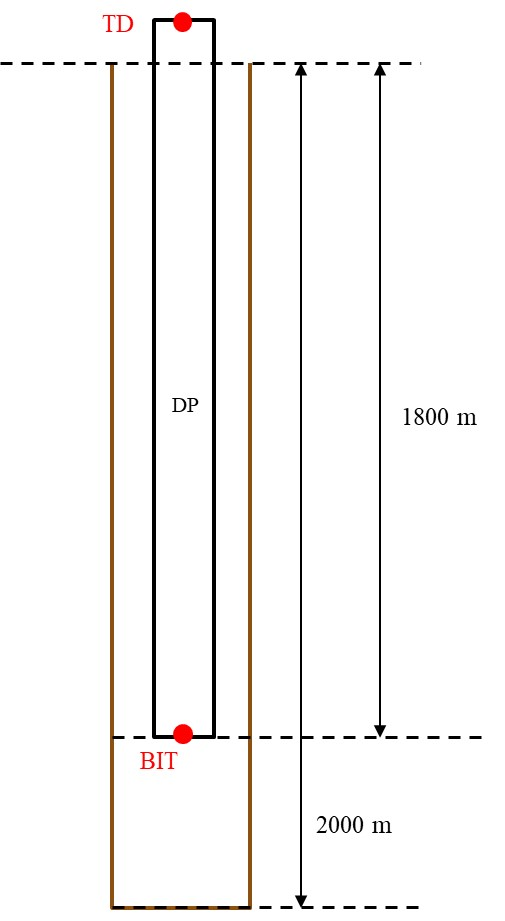
\includegraphics[width=1.5in]{VerticalWellConfig}
  \caption[Schematic of well and drill string for model comparison.]{Schematic of well and drill string for model comparison.}\label{figure_verticalwell}
\end{figure}

\begin{table}[!hbt]
\centering
\begin{tabular}{|c|c|c|c|}
\hline
Parameter & value (imperial units) & value (metric units) & description\\                                                              
\hline
$\rho$ & $490.6\;lb/ft^3$ & $7850\;kg/m^2$ & Drill pipe density \\                                                  
\hline
G & $1.67e^9\;lbf/ft^3$ & $7.99e^{10}\;Pa$  & Shear modulus \\                                                  
\hline
OD & 5.88 in & 0.15 m & drill pipe outer diameter\\                                                       
\hline
ID & 5.00 in & l.127 m & drill pipe inner diameter  \\                                                      
\hline
MD & 6561 ft & 2000 m & measured depth\\                                                              
\hline
TVD & 6561 ft & 2000 m & total vertical depth\\
\hline
Bit depth & 5905 ft & 1800 m & - \\ 
\hline
\end{tabular}
\caption[Well survey data for model comparison (vertical well)]{Well survey and drill string data for model comparison (vertical well without BHA components)}\label{table_verticalwell_input}
\end{table}
The test was conducted by assuming the top drive velocity to be increased from 0 RPM to 40 RPM at 1 second and maintained the velocity for rest of the time. The top drive velocity is shown in \figurename~\ref{figure_topdrive_VSP}

\begin{figure}[!hbt]
  \centering
  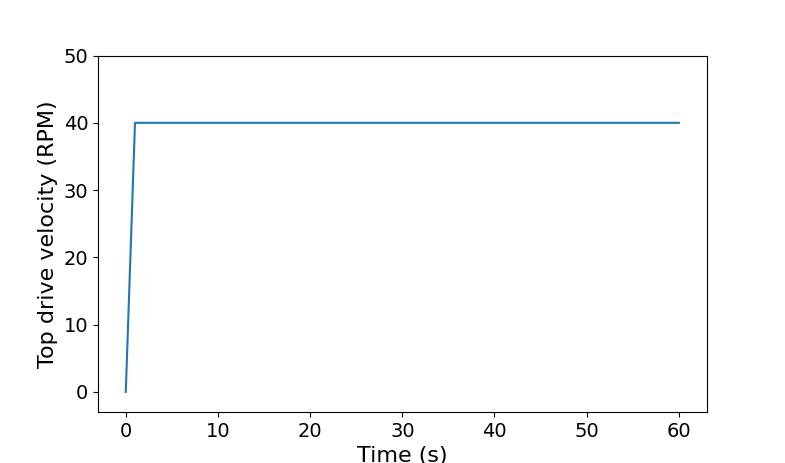
\includegraphics[width=3in]{TopdriveVSP}
  \caption[Top drive set velocity]{Top drive set velocity}\label{figure_topdrive_VSP}
\end{figure}

Before comparing between the models, the PI-controller of the top drive in PYTHON ver. was eliminated since it was sensitive to input parameter which are $k_e, k_i, J_{TD}$, and ramp speed (\tablename~\ref{AS_inptut_params}). \figurename~\ref{figure_topdrive_sensitivity} illustrates the comparison between MATLAB ver. and PYTHON ver. when same parameters were used for top drive (\tablename~\ref{table_topdrivesensitivity_input}). Please note that the absolute value is different because of the unit differences.

\begin{figure}[!hbt]
  \centering
  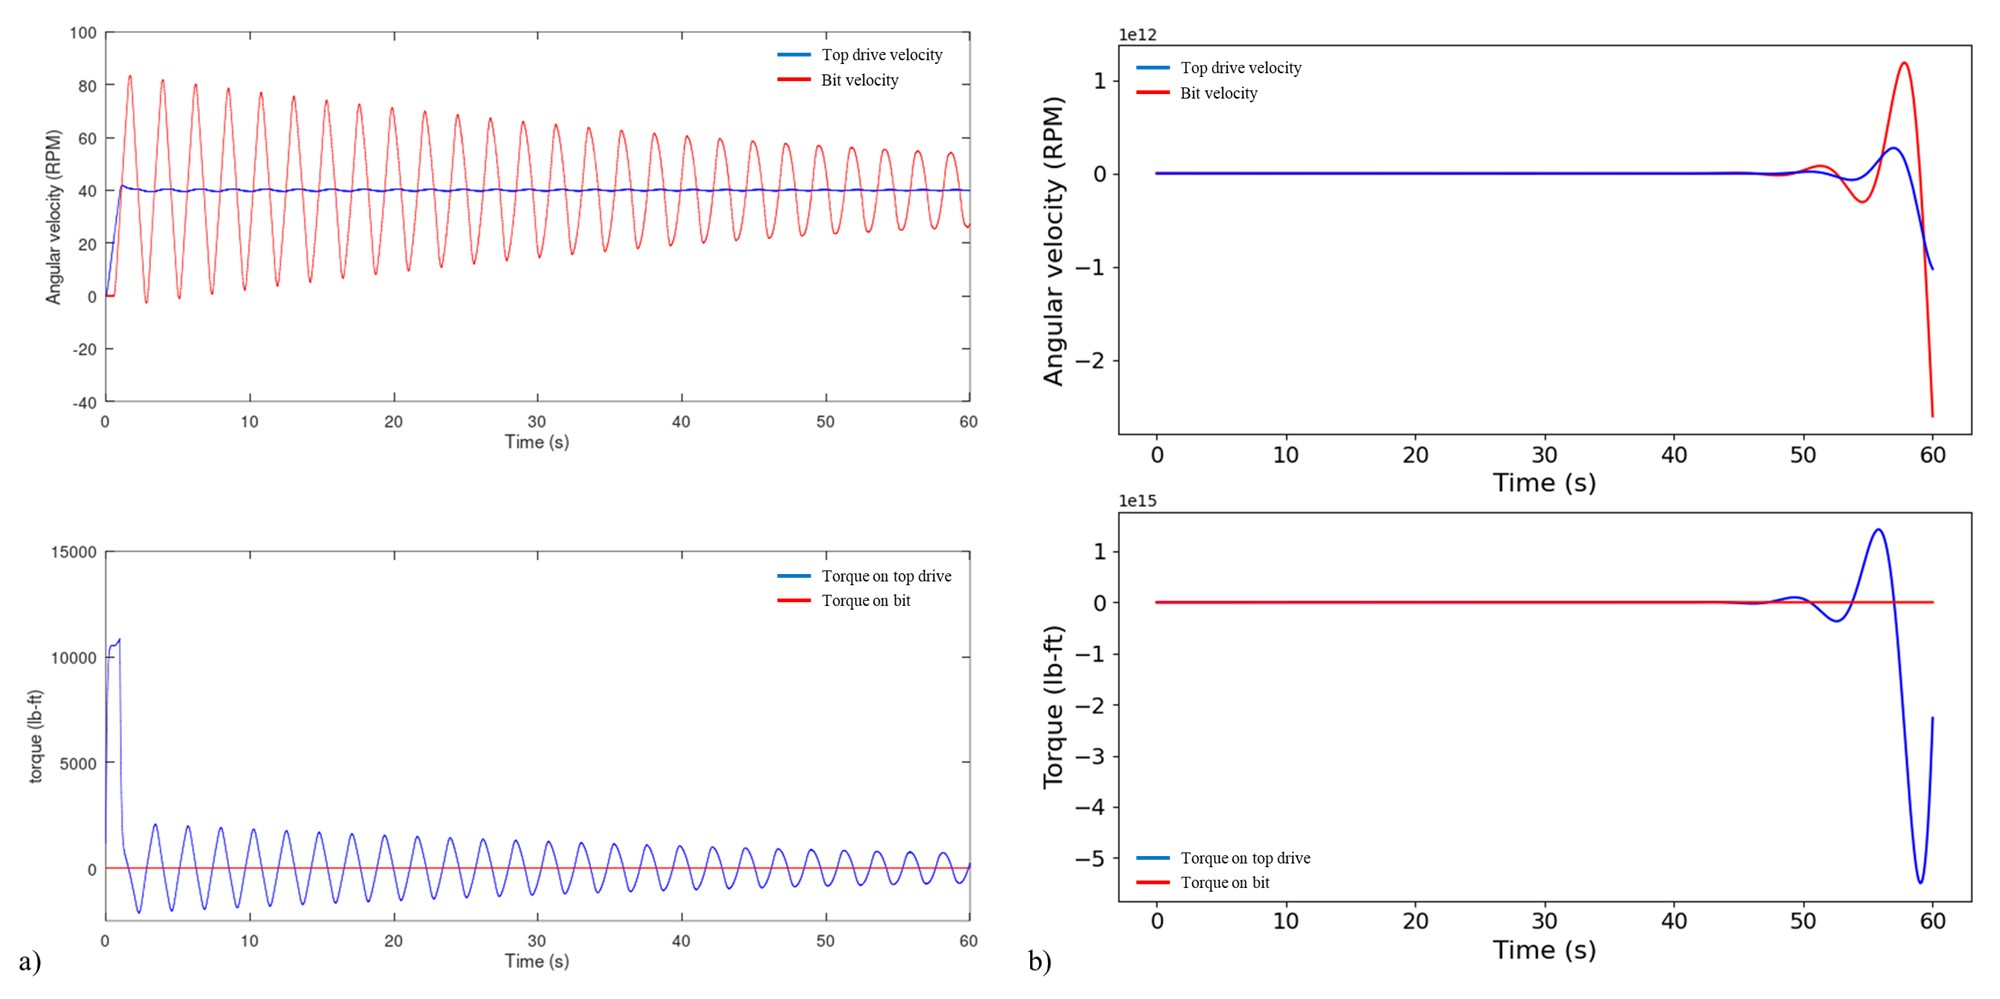
\includegraphics[width=6in]{verticalwell_topdrive_sensitivity}
  \caption[Comparison of drillstring response to same top drive parameters]{Comparison of top drive and bit responses with same top drive parameters between MATLAB ver. and PYTHON ver. a): Results from MATLAB ver., and b) : results from PYTHON ver.}\label{figure_topdrive_sensitivity}
\end{figure}

\begin{table}[!hbt]
\centering
\begin{tabular}{|c|c|c|c|}
\hline
Parameter & value (imperial units) & value (metric units) & description\\                                                              
\hline
$\rho$ & $490.6\;lb/ft^3$ & $7850\;kg/m^2$ & Drill pipe density \\                                                  
\hline
G & $1.67e^9\;lbf/ft^3$ & $7.99e^{10}\;pa$  & Shear modulus \\                                                  
\hline
OD & 5.88 in & 0.15 m & drill pipe outer diameter\\                                                       
\hline
ID & 5.00 in & l.127 m & drill pipe inner diameter  \\                                                      
\hline
MD & 6561 ft & 2000 m & measured depth\\                                                              
\hline
TVD & 6561 ft & 2000 m & total vertical depth\\
\hline
Bit depth & 5905 ft & 1800 m & - \\ 
\hline
\end{tabular}
\caption[Well survey data for model comparison (vertical well).]{Well survey and drill string data for model comparison (vertical well without BHA components.)}\label{table_topdrivesensitivity_input}
\end{table}

To acquire stable behavior of the drill string from PYTHON ver., parameter tuning was conducted. After finding the proper top drive PI-controller parameters, we also modified the code which removes the top drive assuming the fixed velocity at the top of the drill string. This is to reduce the parameters of the model for more simple comparison between different models for the future work. The flowchart of PI-controller removal is shown in \figurename~\ref{figure_Topdriveremove_math}.
\begin{figure}[!hbt]
  \centering
  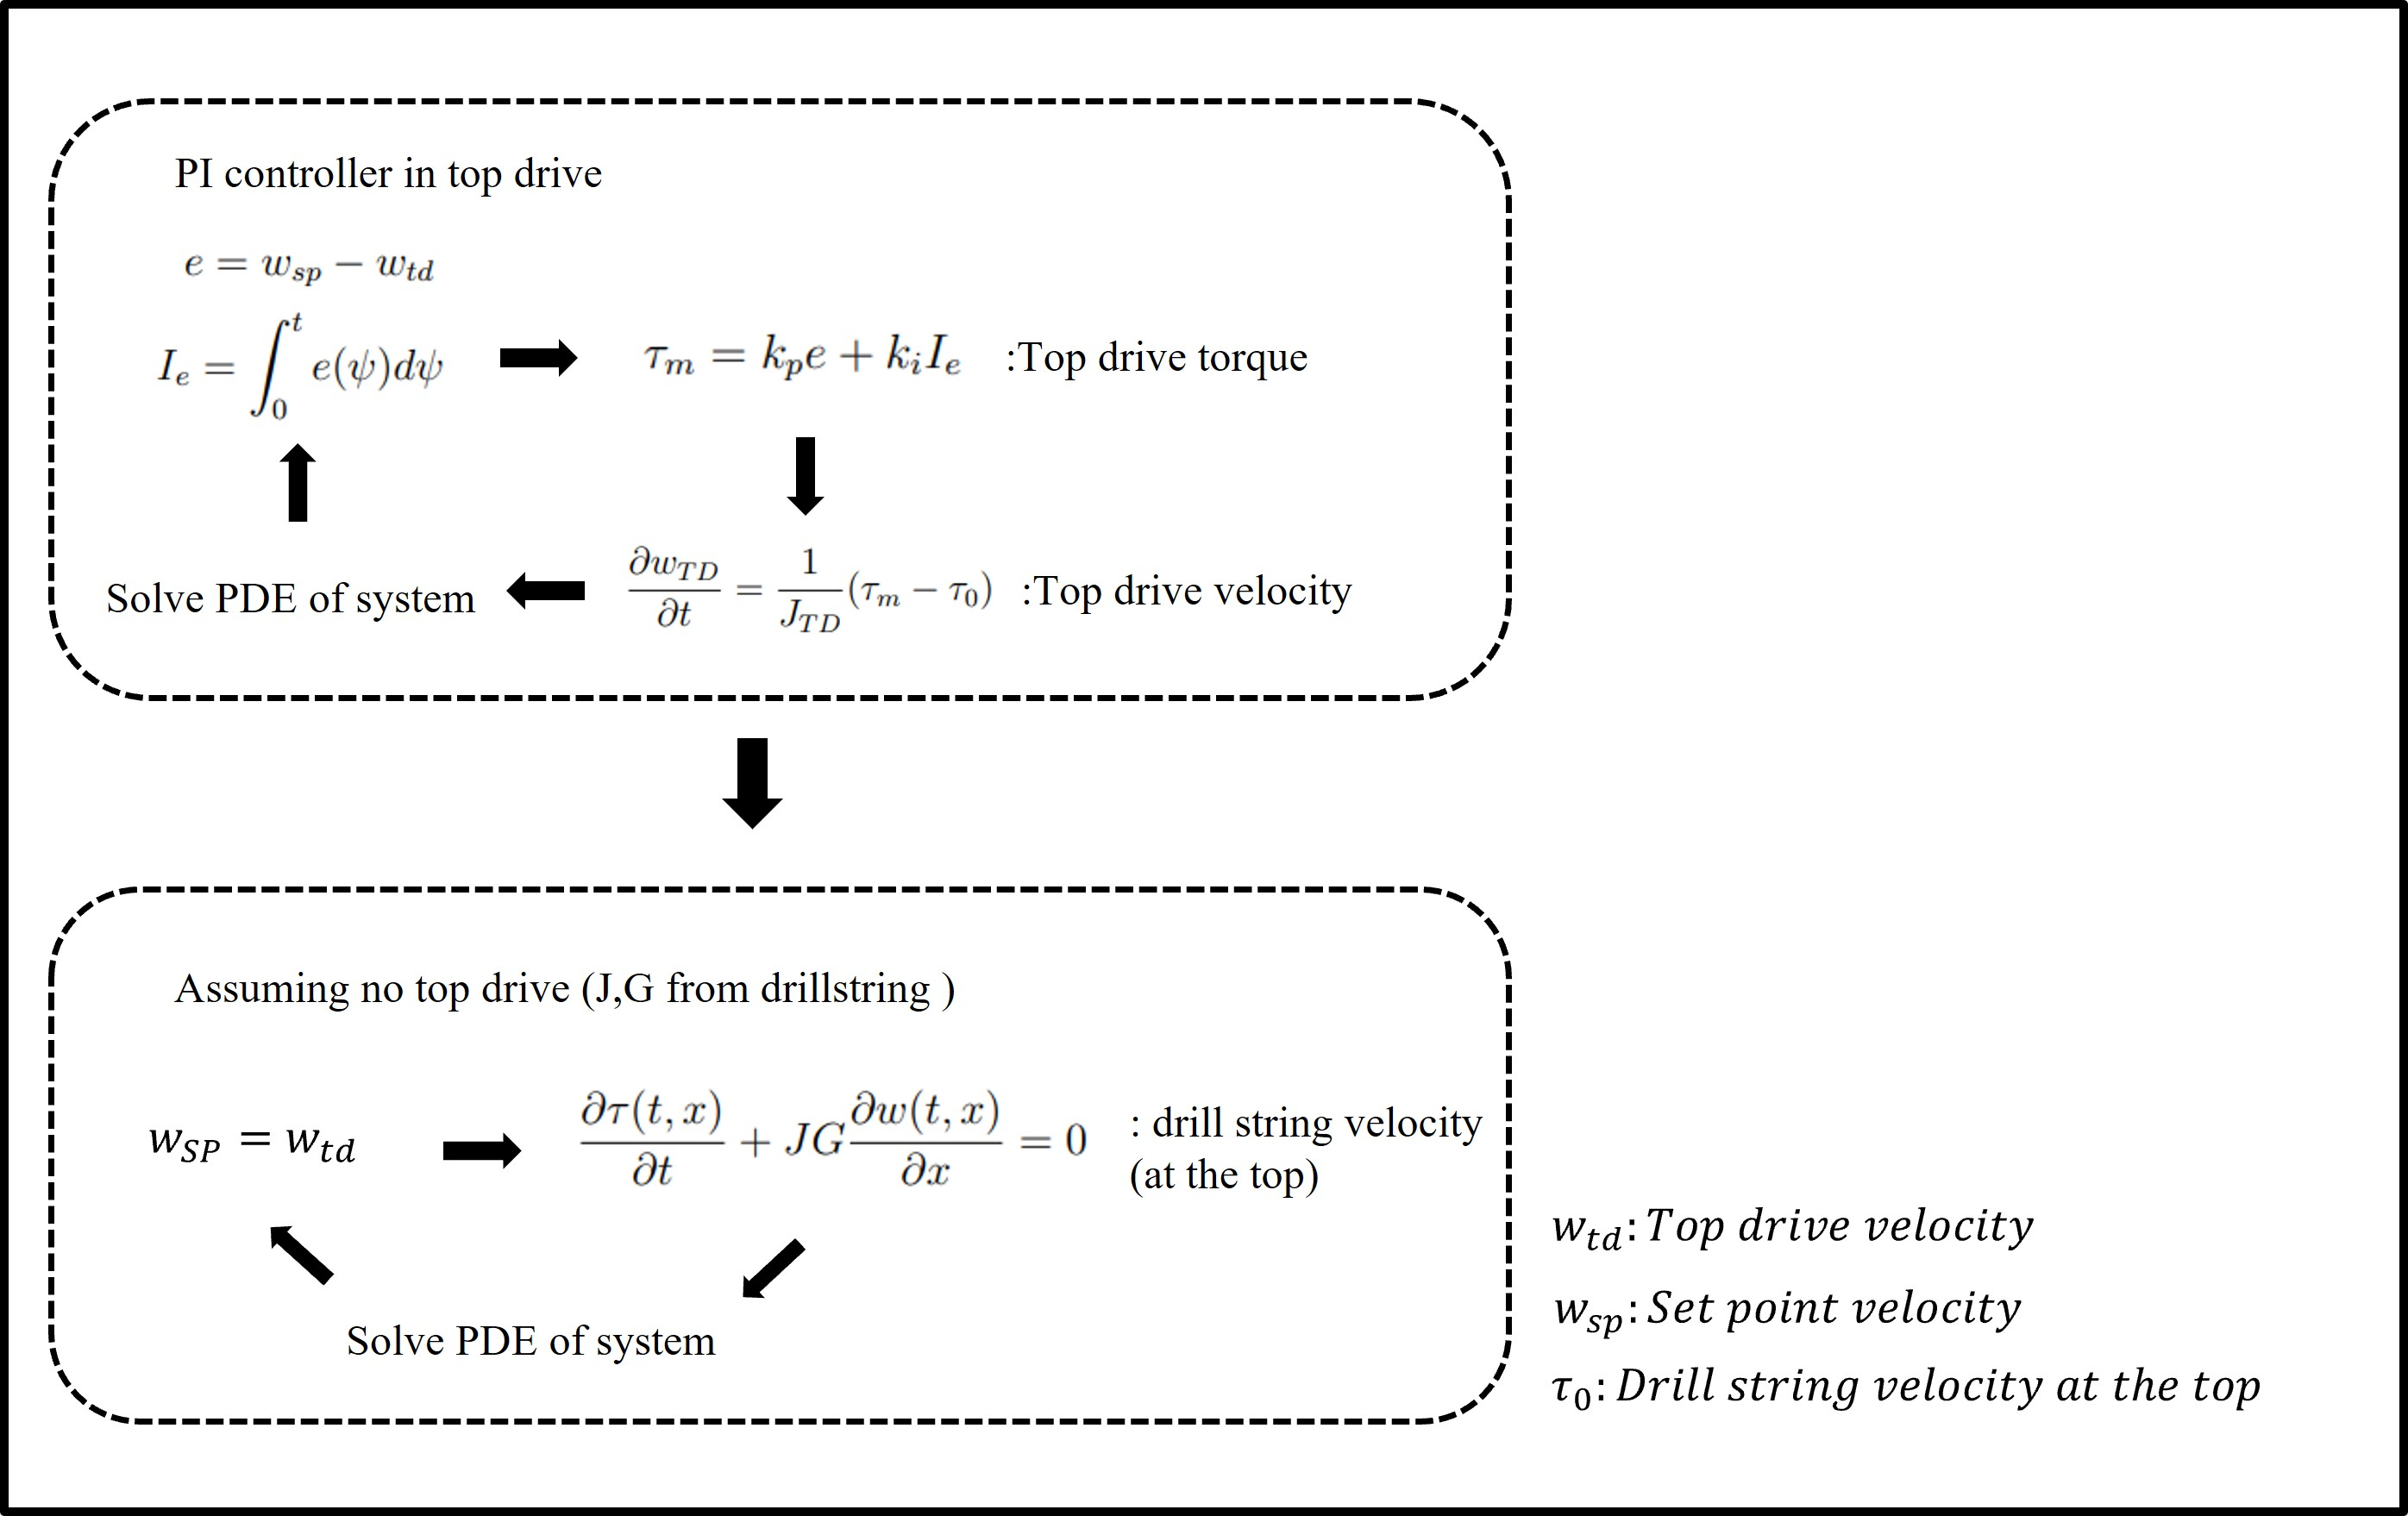
\includegraphics[width=6in]{Topdriveremove_math}
  \caption[flow chart of top drive elimination]{Flow chart of top drive elimination. The modification of the model assumes only drill string in the model and it rotates with given (fixed) velocity at the top of the drill string.}\label{figure_Topdriveremove_math}
\end{figure}

The comparison of bit and top drive angular velocity and torque between when the top drive is existed and removed are depicted in \figurename~\ref{figure_topdriveremove}. In the modified code, top drive velocity and torque will refer that of top of the drill string. Both showed same behavior except during the very first stage when the top drive velocity increased from 0 to 40 RPM. The spikes can be seen when the top drive with PI-controller exits. 

\begin{figure}[!hbt]
  \centering
  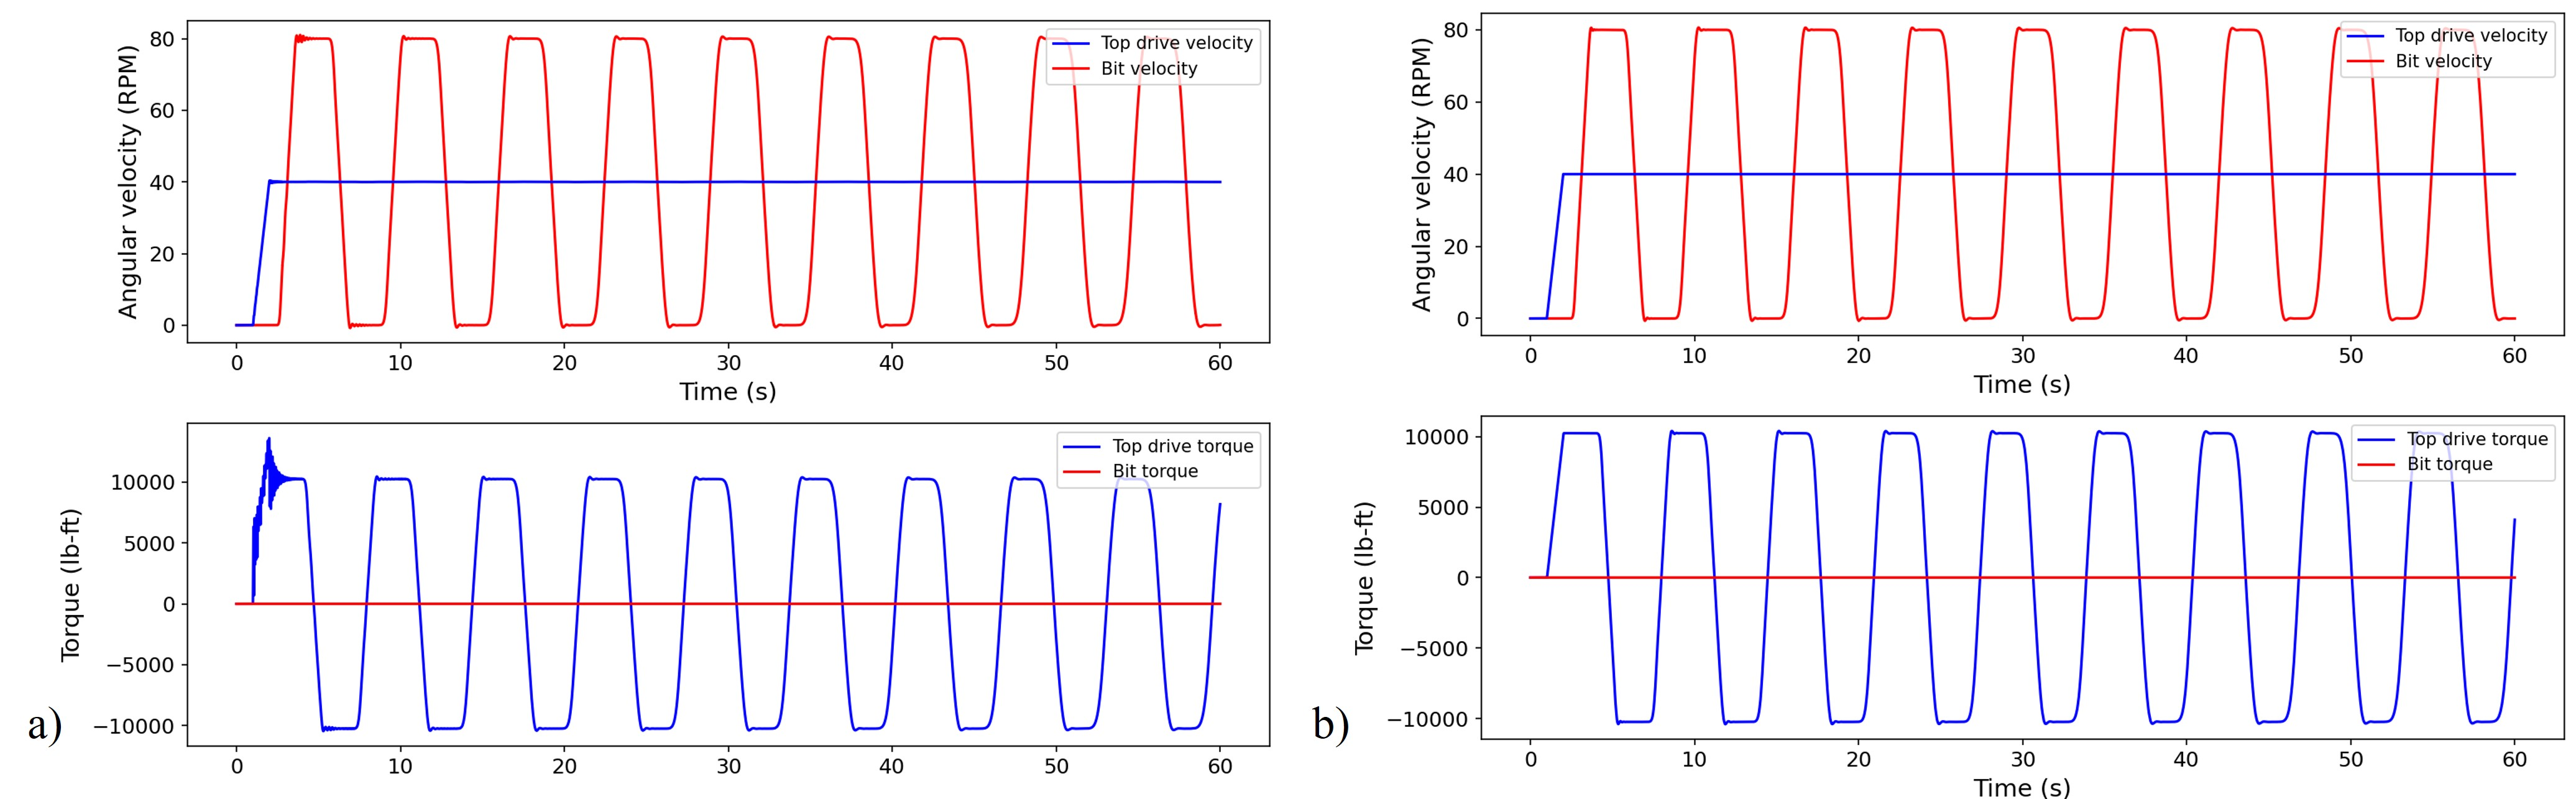
\includegraphics[width=6.5in]{Topdriveremove}
  \caption[comparison between with and without top drive]{Comparison of the angular velocity and torque of the top drive and bit when top drive with and without top drive. a): Response with top drive, b): response without top drive (only drill string).}\label{figure_topdriveremove}
\end{figure}

Interestingly, in both cases, there was a period where angular velocity of the bit was maintained at maximum value for about 2 seconds. The duration that the bit maintains the angular velocity was reduced by increasing the top drive velocity smoothly. The effect of how the top drive velocity increases are illustrated in \figurename~\ref{figure_topdriveveleffect}.

\begin{figure}[!hbt]
  \centering
  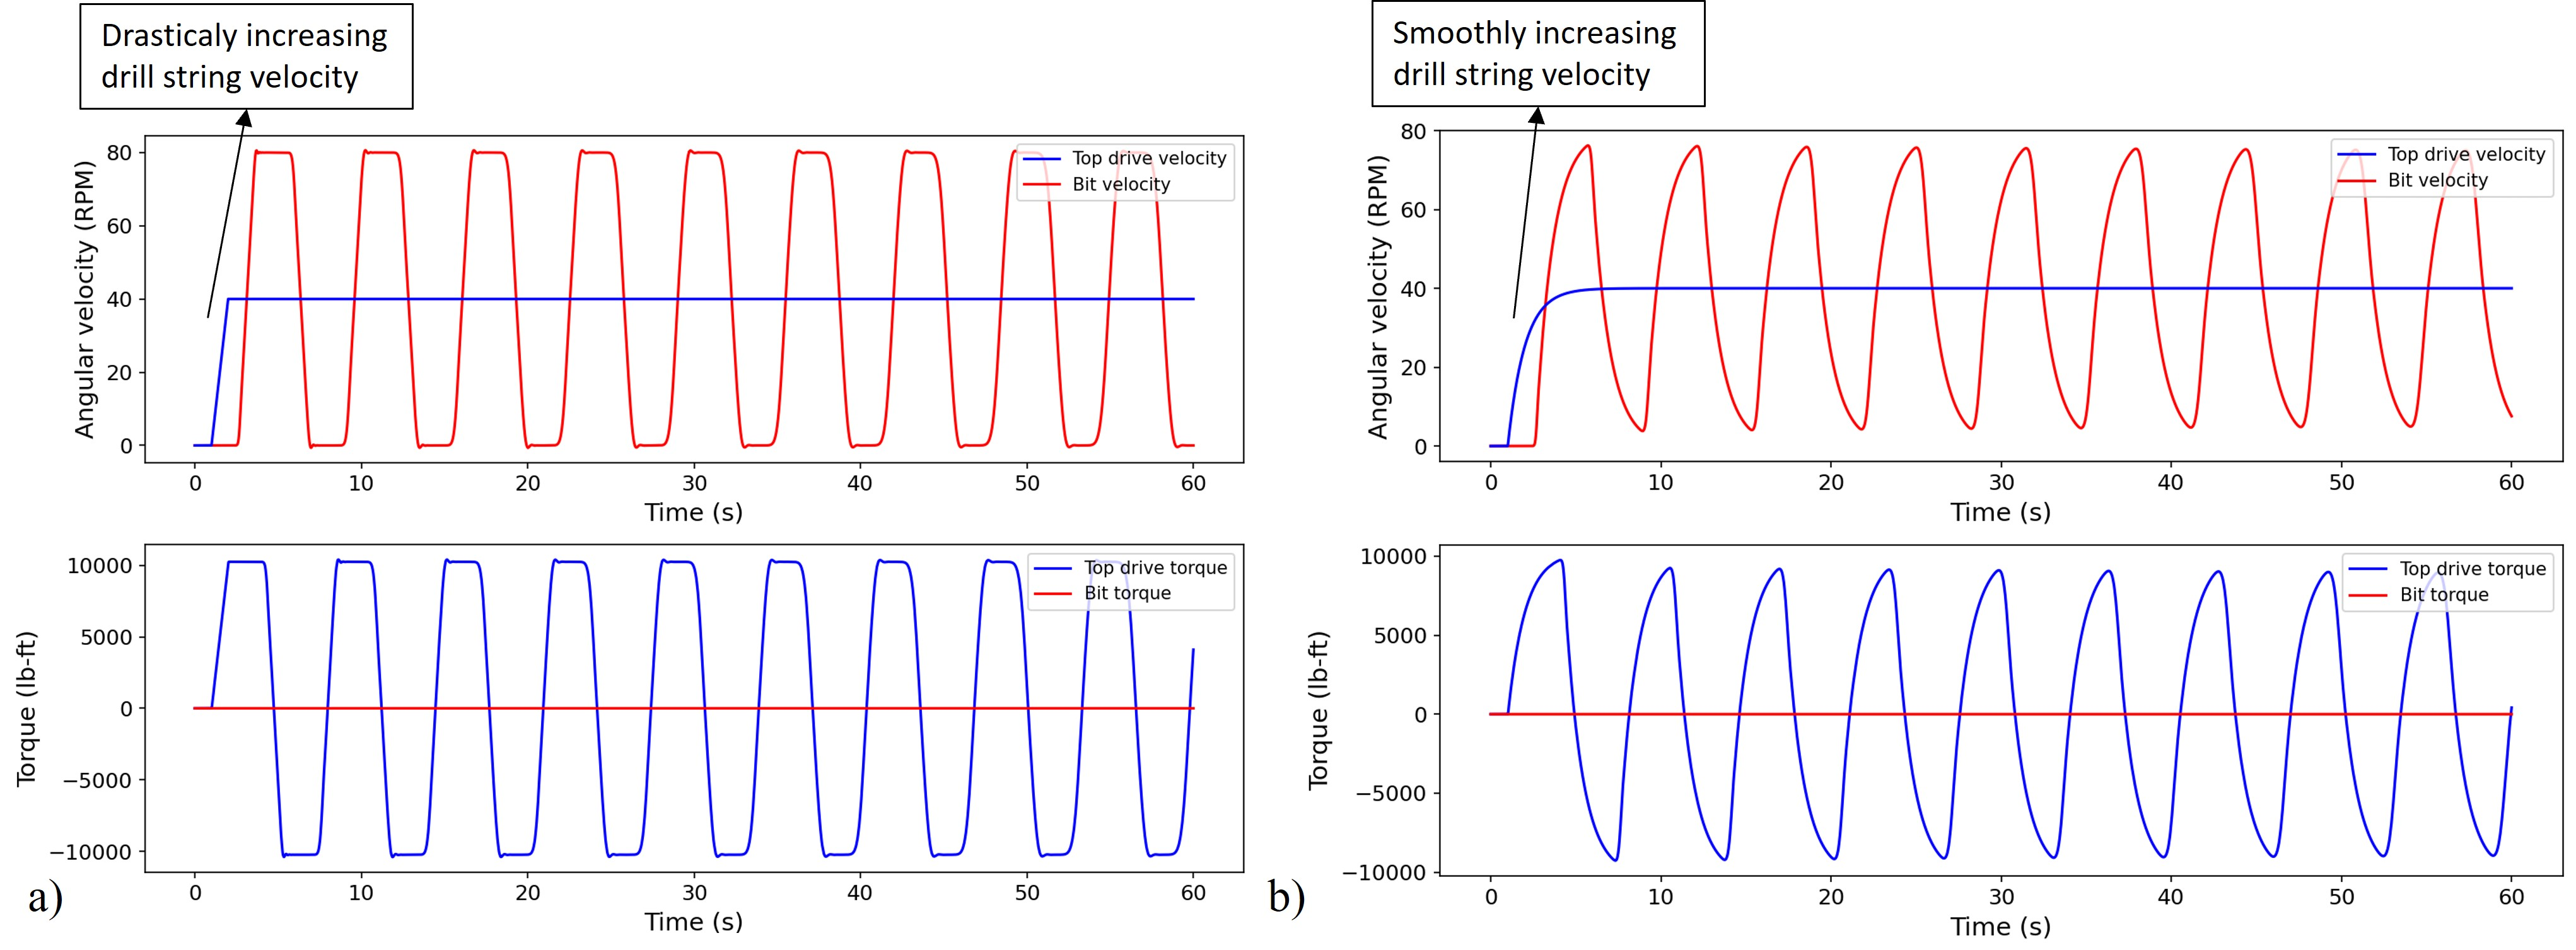
\includegraphics[width=6.5in]{topdriveveleffect}
  \caption{Effect of top drive velocity increasing method. When the velocity increased to set point velocity a): drastically, and b): smoothly.}\label{figure_topdriveveleffect}
\end{figure}

Comparison between A-S model (both Matlab ver. and Python ver.), and Exxon mobil model was conducted with given input in \tablename~\ref{table_verticalwell_input}. The modified code of PYTHON ver. with removed top drive was used for the comparison. First, for the simplicity, the viscous damping was assumed to be zero. Moreover, the coulomb friction is also zero since there is no contact between drill string and borehole (vertical well). Therefore the source term of the governing equation will be zero in equation \equationname~\ref{AS-motion} and the parameters that affects the model will be the density, shear modulus of drill pipe.

The comparison between different models are shown in \figurename~\ref{figure_modelcomparison_vertical_torque}. As can be seen from the results all the model showed  oscillation of the top drive torque, however, significant difference were observed in A-S model PYTHON ver. while MATLAB ver., and exxon mobil model shwed maximum torque about 2000 lb-ft, torque of the PYTHON ver. reached 10,000 lb-ft. Also, the differences in the oscillation frequencies were observed. The frequency of oscillation were 0.32, 0.45, and 0.125 for MATLAB ver., and Exxon mobil model, and PYTHON ver., respectively. Although MATLAB ver. and Exxon mobil model showed similar response, the convergence time of this oscillation were significantly shorter in MATLAB ver. The comparison of the converging time between MATLAB ver. and PYTHON ver. is illustrated in \figurename~\ref{figure_modelcomparison_vertical_convergence}. The comparison of the model are summerized in Table....

\begin{figure}[hbt!]
  \centering
  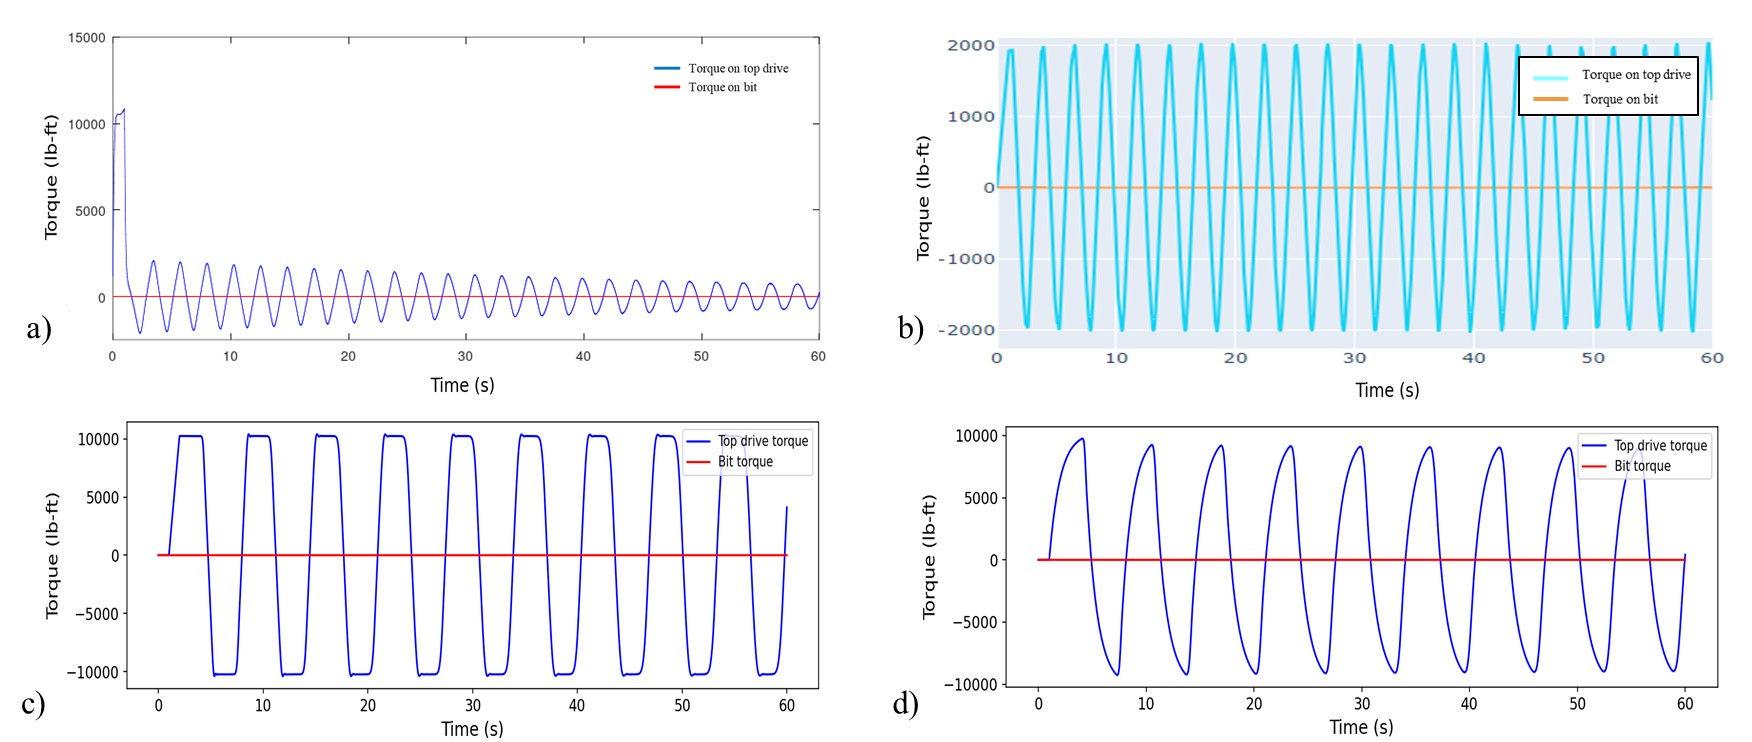
\includegraphics[width=6in]{modelcomparison_vertical_torque}
  \caption[Comparison of torque of top drive and bit without viscous damping and BHA components in vertical well]{Comparison of torque of top drive and bit without viscous damping and BHA components in vertical well. the input parameteres for drill string is summarized in \tablename~\ref{table_verticalwell_input}. a): A-S model (MATLAB ver.), b): Exxon mobil model, c) A-S model (PYTHON ver.), and d): A-S model (PYTHON ver.) with smooth increase of top drive velocity.}\label{figure_modelcomparison_vertical_torque}
\end{figure}

\begin{figure}
  \centering
  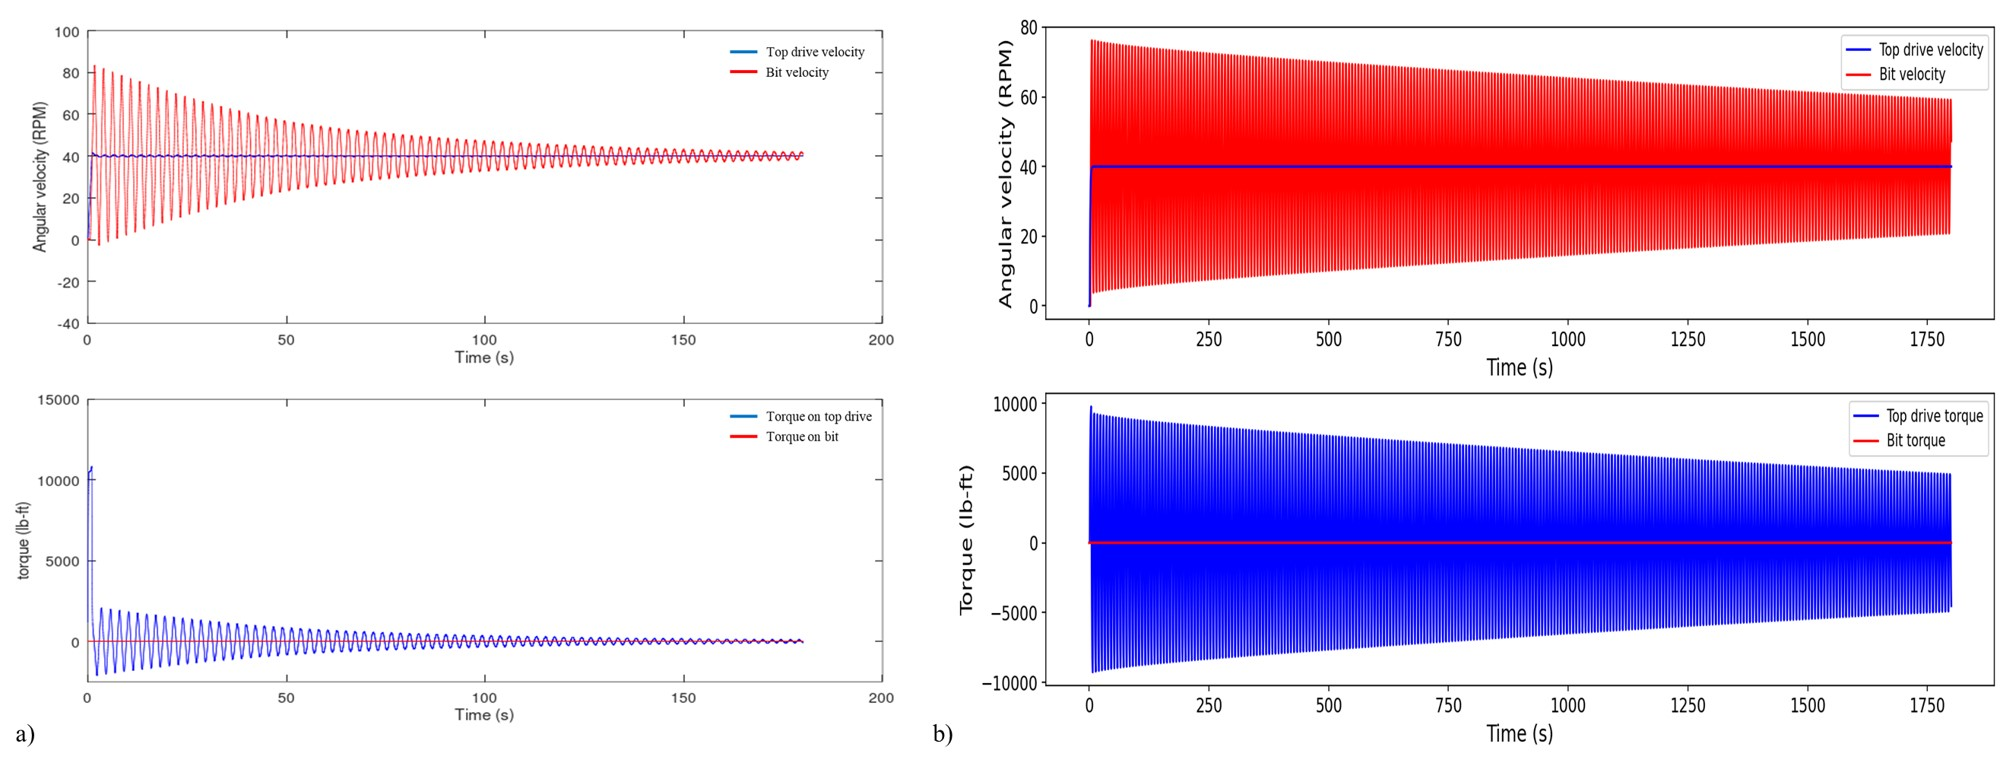
\includegraphics[width=6.5in]{modelcomparison_vertical_convergence}
  \caption[Comparison of torsional vibration convergence time without viscous damping and BHA components in vertical well.]{Comparison of torsional vibration convergence time without viscous damping and BHA components in vertical well. a): A-S model MATLAB ver., b): A-S model PYTHON ver.}\label{figure_modelcomparison_vertical_convergence}
\end{figure}

%\begin{table}[!hbt]
%\centering
%\begin{tabular}{|c|c}|c|c|}
%\hline
% & Exxon mobil model & A-S model (MATLAB ver.) & A-S model (PYTHON ver.) \\                                                              
%\hline
%Drill string vibration convergence & - & $<$ 150s & $>$ 30min \\                                                  
%\hline
%Vibration frequency & 0.32 & 0.45  & 0.125 \\                                                  
%\hline
%Maximum torque on top drive (lb-ft) & 2000 in & 2000 & \\                                                       
%\hline
%\end{tabular}
%\caption[Summary of model comparison without damping and BHA components in vertical well.]{Summary of model comparison without damping and BHA components in vertical well.}\label{table_modelcomparison_vertical_input}
%\end{table}

\newpage
\subsection{Case 2 - Inclined well}

The model was tested with inclined well with simple configuration of drill string. The MD of the well is 4000 m with 60 deg inclination. The drill bit is off-bottom where located at 2500 m depth. The Schematic view of wellbore and drill string are depicted in \figurename~\ref{figure_wellconfig_inclined}. Also, the top drive velocity is increased to 40 RPM at 1 second which is same with test case 1 (\figurename\ref{figure_topdrive_VSP}). For test case 2, the viscous damping is neglected for the simplicity of the test. However, Coulomb friction is considered to investigate the stick-slip occurrence during drilling. The parameters for the test are summarized in \tablename~\ref{table_Inclinedwell_input}.

\begin{figure}[!hbt]
  \centering
  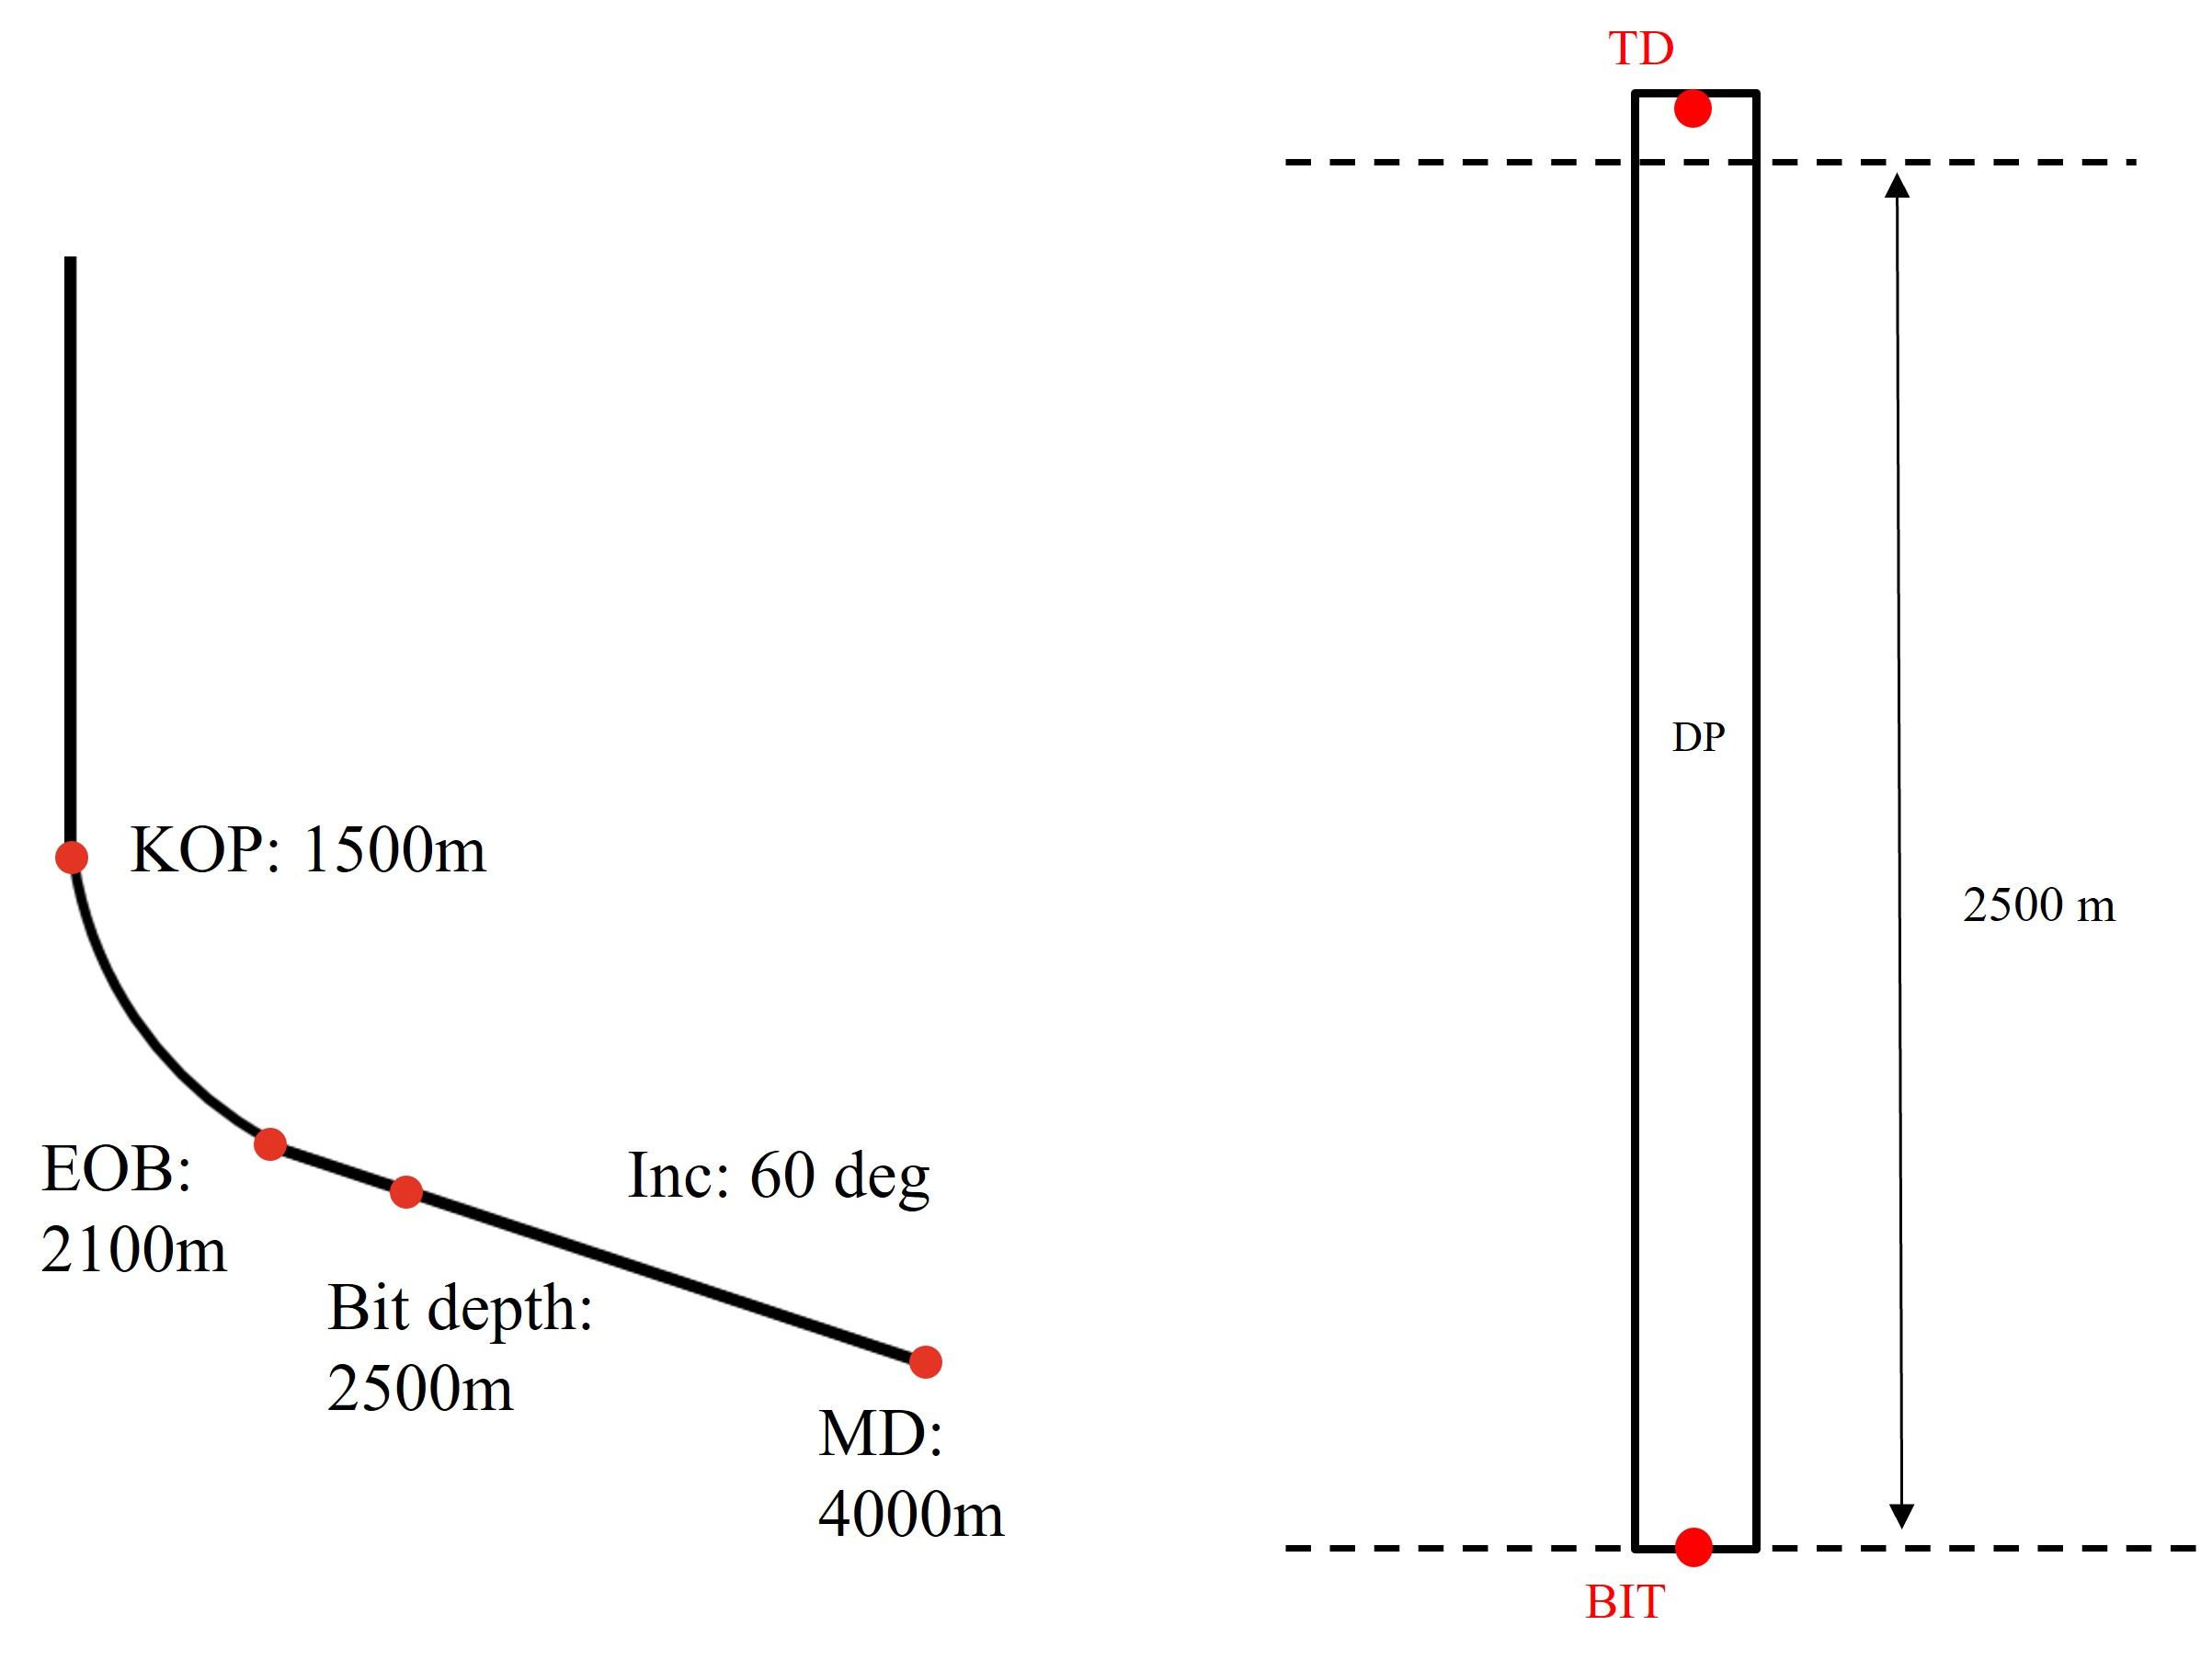
\includegraphics[width=4in]{InclinedWellConfig}
  \caption[Schematic view of test case 2.]{Schematic view of wellbore and drill string for test case 2.}\label{figure_wellconfig_inclined}
\end{figure}

 \begin{table}[!hbt]
\centering
\begin{tabular}{|c|c|c|c|}
\hline
Parameter & Value (imperial units) & Value (metric units) & description\\                                                              
\hline
$OD_{dp}$ & 5.88 in & 0.15 m & drill pipe outer diameter\\                                                       
\hline
$ID_{dp}$ & 5.00 in & 0.l127 m & drill pipe inner diameter  \\                                                      
\hline
$\rho_{dp}$ & $490.6\;lb/ft^3$ & $7850\;kg/m^2$ & Drill pipe density \\                                                  
\hline
$G_{dp}$ & $1.27e^{9}\;lb/ft^3$ & $6.10e^{10}\;pa$ & drill pipe shear modulus\\                                                              
\hline
$\mu$ & 0.5 & 0.5 & Static friction factor\\
\hline
$fRat$ & 0.5 & 0.5 & Static friction/Dynamic friction\\
\hline
$w_c$ & 10 RPM & 10 RPM & Cut-off angular velocity\\
\hline
\end{tabular}
\caption[Input parameters for test case 2.]{Input parameters for test case 2. fRat only included in MATLAB ver. model, have to figure how to convert it to dynamic friction factor***).}\label{table_Inclinedwell_input}
\end{table}

The results from A-S models are shown in \figurename~\ref{figure_testcase2_ASmodel}. Both model captured the stick-slip event during of-bottom drill string rotation. However, similar to test case 1 (have to rename it later: vertical well test), the top drive torque amplitude and the frequency of the oscillation showed significant differences.
 
\begin{figure}[!hbt]
  \centering
  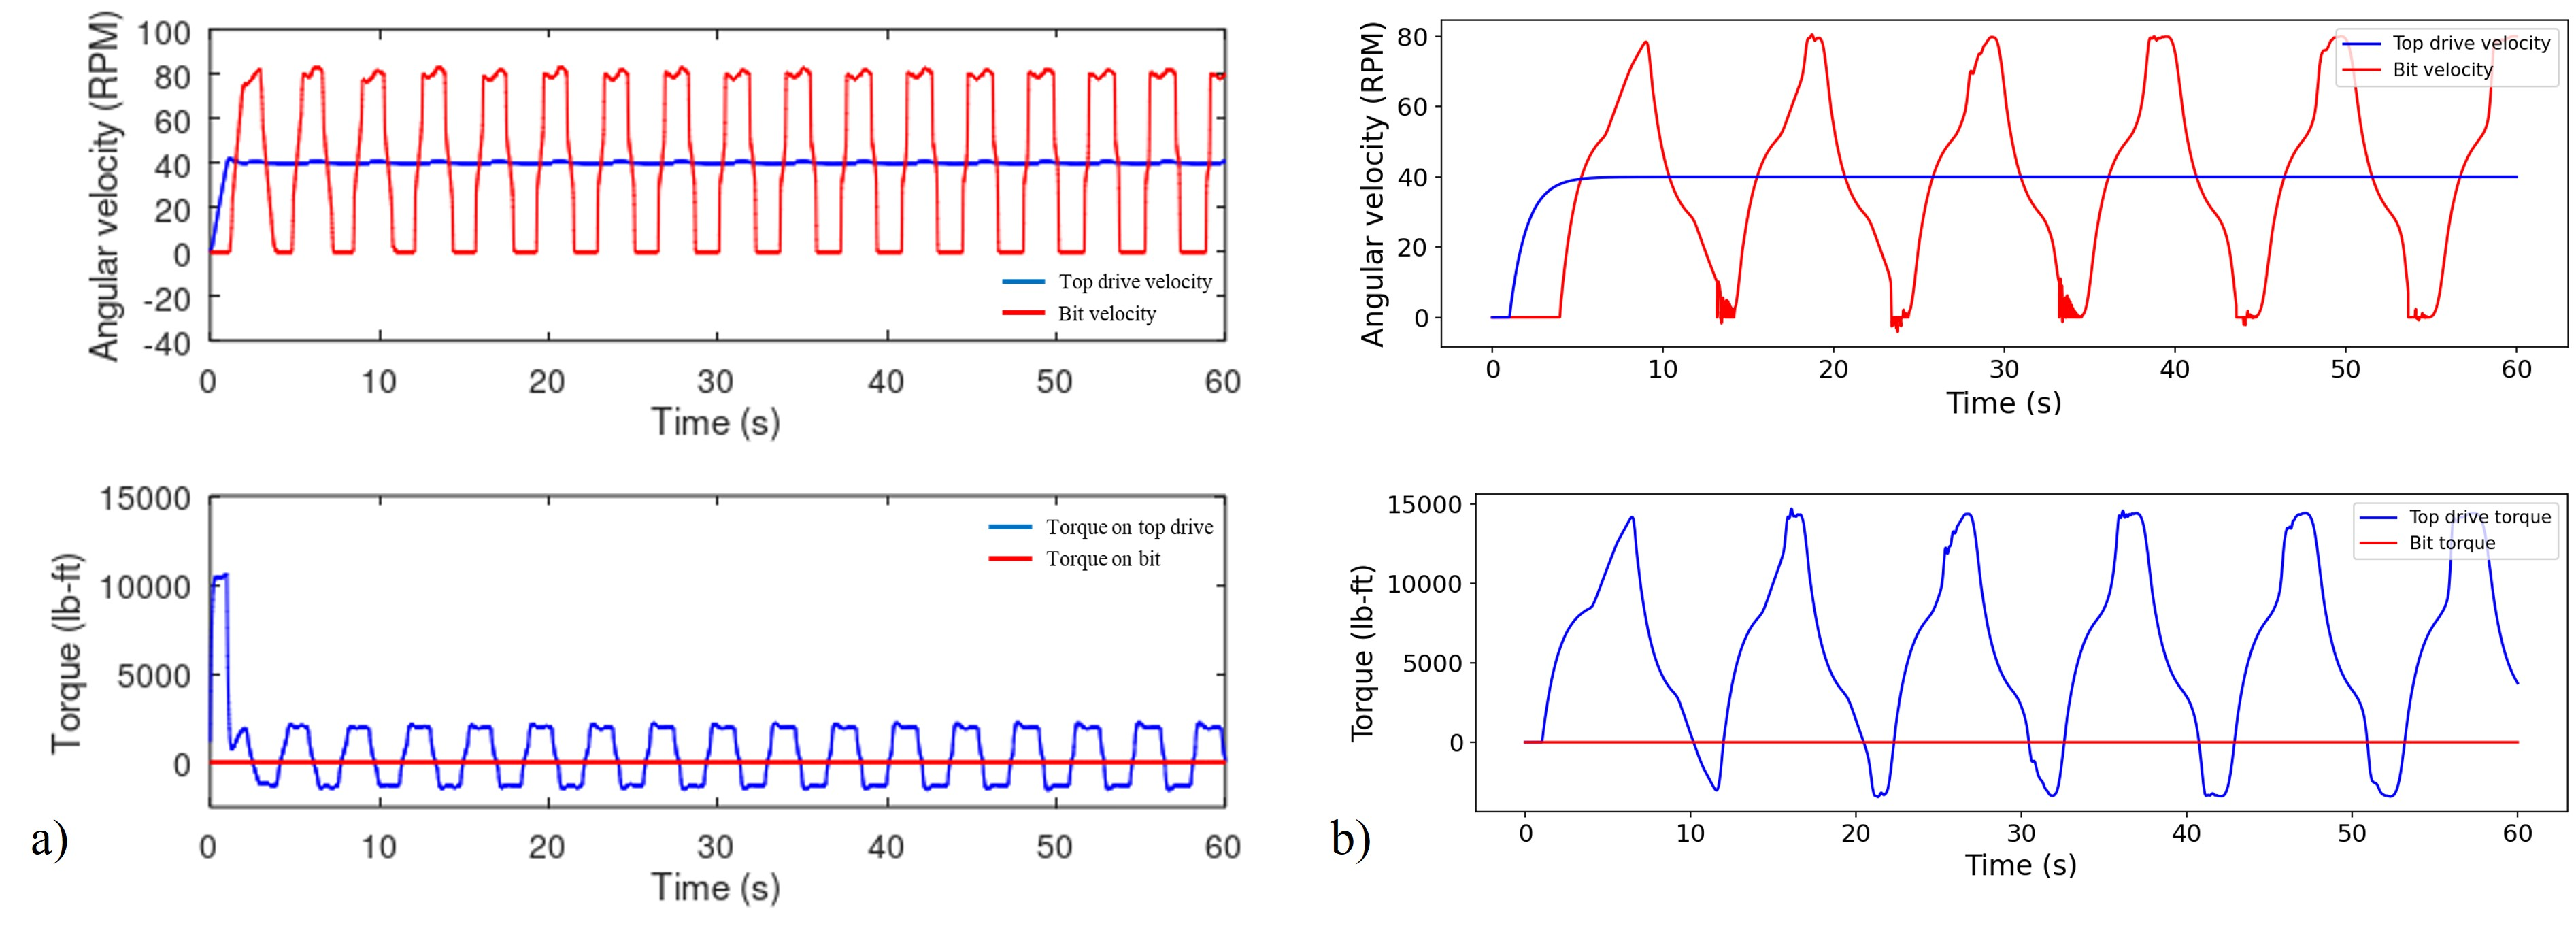
\includegraphics[width=6.5in]{Testcase2_ASmodel}
  \caption[Result from A-S model. (test case 2)]{Simulation results of A-S model for test case 2, a): MATLAB ver, and b): PYTHON ver. Stick-slip was observed from the model.}\label{figure_testcase2_ASmodel}
\end{figure}


A-S model
\begin{numberedlist}
	\item Difference in torque amplitude
	\item Difference in oscillation frequencies
	\item Bit model - constant torque
	\item Comparison using color map?
\end{numberedlist}

\newpage
\subsection{Case 3 - Vertical Well with BHA}

\begin{figure}[!hbt]
  \centering
  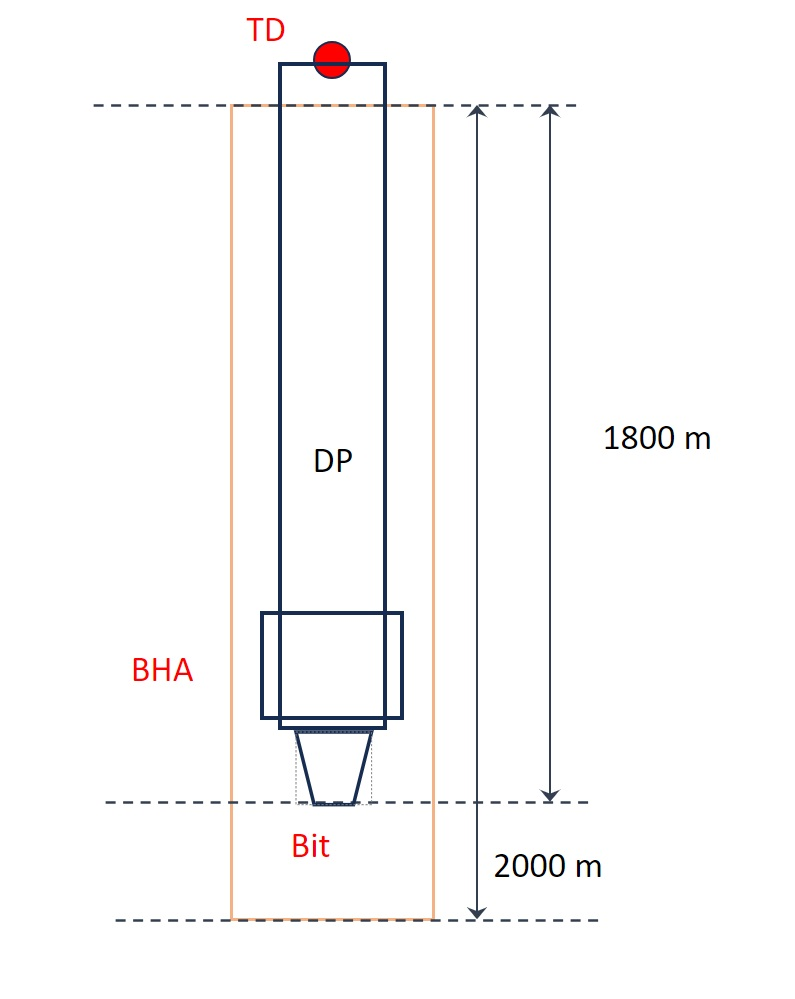
\includegraphics[width=2in]{VerticalWellConfigBHA}
  \caption{Schematic of well and drill string for model comparison}\label{Vert_well_conf_BHA}
\end{figure}


\begin{table}
  \centering
  \begin{tabular}{|c|c|c|c|}
    \hline
    % after \\: \hline or \cline{col1-col2} \cline{col3-col4} ...
    Parameter & Value (imperial units) & Value (metric units) & Description \\
    \hline
    $OD_{HWDP}$ & 4.50 in & 0.1143 m & Heavy weight drill pipe outer diameter \\
    \hline
    $ID_{HWDP}$ & 2.50 in & 0.0635 m & Heavy weight drill pipe inner diameter \\
    \hline
    $OD_{DC}$ & 6.00 in & 0.1524 m & Drill collars outer diameter \\
    \hline
    $ID_{DC}$ & 2.00 in & 0.0508 m & Drill collars inner diameter \\
    \hline
    $\rho_{dp}$ & 490.6 $lb/ft^{3}$ & 7850 $kg/m^{3}$ & Drill pipe density \\
    \hline
    $G_{dp}$ & 1.27$e^{9}\;lb/ft^{2}$ & 6.08$e^{10} pa$ & Drill pipe shear modulus \\
    \hline
  \end{tabular}
  \caption{Input parameters of BHA for test case 3}\label{Input Parameters TC3}
\end{table} 

In this specific scenario, an additional configuration of the drill string included a Bottom Hole Assembly (BHA). The BHA introduced extra components, resulting in an increase in both the weight and size of the drill string. However, the well survey data for the vertical well remained the same, except for the incorporation of the BHA. The well design, depicted in \figurename~\ref{Vert_well_conf_BHA}, remained unchanged, while the parameters for the top drive were kept constant. For the sake of simplicity, the influence of viscous damping was disregarded. The specific input parameters can be found in the provided \tablename~\ref{Input Parameters TC3}.

After running the simulation we get the following results. Top-drive torque remains constant while Rotational speed of the drill bit plays around

